\documentclass[12pt]{ctexart}
\usepackage{graphicx}
\usepackage{longtable}
% \usepackage{xcolor}
% \usepackage{framed}
% \newenvironment{TODO}
%   {\begin{framed}\color{red} \textbf{TODO:}}
%   {\end{framed}}

\usepackage{booktabs}
\usepackage{graphicx}
\usepackage{float}
\usepackage{dblfloatfix}  % 增强对双栏浮动对象的支持
\bibliographystyle{unsrt} % 使用 unsrt 样式
% 调整 figure 环境的上下间距
\usepackage{setspace}
\setlength{\textfloatsep}{1pt} % 图像与文本之间的距离
\setlength{\floatsep}{5pt} % 图像与图像之间的距离
\setlength{\intextsep}{1pt} % 文本与嵌入图像之间的距离
\usepackage{caption} % 引入caption包以便于使用subcaption宏包
\usepackage{subcaption} % 引入子标题宏包
\usepackage{booktabs} % 支持三线表格
\usepackage{float}    % 用于控制浮动体的位置
\usepackage{titlesec} % 用于标题格式自定义
% 自定义附录标题的格式
\usepackage{appendix}%加入附录需使用appendix宏包
% 自定义附录标题的格式
% 自定义附录标题的格式
\newcommand{\appendixformat}{
    \par
    \setcounter{section}{0}
    \renewcommand{\thesection}{附录 \Alph{section}}
    \titleformat{\section}[block]
        {\centering\Large\bfseries} % 居中对齐,设置字体大小和粗体
        {附录 \Alph{section}}{1em}{} % 标题内容
}
% 颜色和箱子
% \usepackage[x11names]{xcolor} % 确保这里只有一次调用

% 为 TODO 环境设置颜色
\usepackage{framed}

\usepackage[dvipsnames,svgnames]{xcolor}
\usepackage{tcolorbox}
\tcbuselibrary{skins} % 添加skins库以使用更多皮肤样式

% 数学公式和定理环境设置
\usepackage{amsmath} % 数学公式支持
\usepackage{amsthm} % 定理环境支持
\numberwithin{equation}{section} % 方程编号按 section 区分
\newtheorem{theorem}{定理}[section] % 定理环境定义

% 格式和布局设置
\usepackage{multicol} % 多列布局支持
\setlength{\columnsep}{1cm} % 列间距
\setlength{\columnseprule}{0.4pt} % 列间分界线
\usepackage[a4paper, margin=1.3in]{geometry} % 页面边距设置
\usepackage{xeCJK} % 中日韩文字字体支持
\usepackage{indentfirst} % 首段缩进
\usepackage{setspace} % 行距设置
\usepackage{titlesec} % 标题格式设置
\usepackage{fancyhdr} % 自定义页眉页脚
\usepackage{unicode-math} % Unicode 数学字体支持

% 数学字体设置
\setmathfont{Segoe UI Symbol}

% 页面样式和页眉页脚设置
\pagestyle{fancy}
\fancyhf{} % 清除默认的页眉页脚设置

% 设置页眉的内容
\fancyhead[L]{\textit{\small 基于偏振干涉的微弱磁场测量}} % 标题显示在左侧
\fancyhead[R]{\hfill\thepage} % 页码尽量显示在右侧

% 去掉页眉和页脚的分隔线
\renewcommand{\headrulewidth}{0pt} % 去掉页眉的横线
\renewcommand{\footrulewidth}{0pt} % 去掉页脚的横线

% % 设置页眉内容
% \fancyhead[R]{\thepage} % 页码显示在右侧
% \fancyhead[L]{\textit{\small 基于偏振干涉的微弱磁场测量}} % 标题显示在左侧
% % 标题格式设置
\titleformat{\section}
  {\bfseries\Large} % 一级标题字体加粗,大号
  {\thesection} % 标题编号
  {1em} % 标题编号与文本间距
  {} % 标题文本格式

\titleformat{\subsection}
  {\bfseries\large} % 二级标题字体加粗,大号
  {\thesubsection} % 标题编号
  {1em} % 标题编号与文本间距
  {} % 标题文本格式

% 段落和行间距设置
\setlength{\parskip}{0.5\baselineskip} % 段落间距
\setstretch{1.2} % 行间距设置为1.2倍

% 标题之间的间距设置
\titlespacing*{\section}{0pt}{\baselineskip}{0.5\baselineskip} % 一级标题间距
\titlespacing*{\subsection}{0pt}{0.75\baselineskip}{0.25\baselineskip} % 二级标题间距

% 文档标题、作者、日期
\usepackage{geometry} % 页面边距设置
\usepackage{abstract} % 摘要设置
% 摘要格式设置
\renewcommand{\abstractname}{} % 自定义摘要标题
\renewcommand{\absnamepos}{t} % 摘要标题顶格写


% 页面边距设置
\geometry{a4paper, margin=0.5in}
% 移除摘要段落缩进
\setlength{\absleftindent}{0pt} % 左侧缩进
\setlength{\absrightindent}{0pt} % 右侧缩进
% 自定义文档标题、作者、日期
\title{\vspace*{0in} % 调整标题与页面顶部的距离
\centering\bfseries\Huge 基于偏振干涉的微弱磁场测量} % 标题居中显示
\author{}
\date{}
\begin{document}
\maketitle
\begin{abstract}
     \vspace{-1in} % 调整摘要与标题之间的距离
     \textbf{摘要:}本文详细阐述了一种基于偏振干涉原理的微弱磁场测量技术,该技术主要依托法拉第磁致旋光效应、光自旋霍尔效应以及偏振相消干涉原理。实验采用了包括半导体激光器、偏振片、磁光晶体、透镜和CCD相机在内的一系列设备,以实现在不同环境条件下对磁场强度的精确测量。实验结果证明了所提方法的有效性,测量精度高,理论精度可达$10^{−6}$T,适用于存在可燃性气体等特殊环境。此外,文章还对实验中可能出现的误差来源进行了分析,并通过不确定度分析确保了测量结果的可靠性。该实验装置结构简单、成本低廉、灵活性高,具有广泛的应用前景
    
     \textbf{关键词:} 微弱磁场测量;偏振干涉;法拉第效应;光自旋霍尔效应;高精度测量;误差分析;不确定度
\end{abstract}

\tableofcontents
\newpage
% \begin{multicols}{2}
\section{实验背景}
我国是最早认识磁现象的国家之一,《管子》这部成书于公元前4世纪左右的著作中记载了“上有慈石者,其下有铜金”,这是关于磁的最早记载。磁场广泛存在于空间之中,对于物理世界的影响不言而喻,然而磁场本身无法为肉眼所直接观察,故磁场测量显得尤为重要。磁场传感器作为研究空间磁场的工具,在医疗仪器、矿物勘探等各个领域的应用广泛。常用的磁场测量方法可以分为六大类:磁通门法、霍尔效应法、磁阻效应法、磁共振法、超导效应法和磁光效应法。传统的电学磁场传感器均为电接触式,且对环境敏感,在某些环境条件下,如瓦斯等可燃性气体环境中无法使用。且上述方法或无法实时显示,响应时间长,或存在磁滞回线,干扰测量结果,或体型巨大,价格高昂。

本实验的目的在于通过磁致旋光效应设计一种磁场测量方案,具备实时显示、操作简便、成本低、轻便、高测量精度等优点,并通过实验验证该方案的合理性和可行性。
\section{研究特色}
\begin{enumerate}
    \item 实验原理方面:本实验依据磁致旋光效应和非对称偏振干涉方法,其中磁场在$0$到$9.41*10^{-4}T$测量结果具有较好的线性关系;
    \item 设备特色方面:本实验设备仪器装配简单,造价低廉。实验仪器可拆卸,灵活性高,便于教学演示。
    \item 效率质量上:本实验装置一经装配、调节,可以立即进行连续的磁场测量,且测量时间短、测量精度高(理论精度可以达到$10^{-6}T$)。
    \item 应用对象上:该实验装置能够精确测量各种环境下的磁场,尤其适用于充满可燃性气体等环境条件下的磁场测量。与传统的磁场测量方法相比,该装置无需在环境中使用电力,从而确保了安全性。
    \item 应用范围的拓展:该方案中的磁光晶体可替换为其他光学调制器件,从而实现多种物理参量的精密测量。
\end{enumerate}
\section{实验原理}
\subsection{法拉第磁致旋光效应}
\begin{figure}[H] % h! 表示“尽可能在当前位置插入”
    \centering % 图片居中
    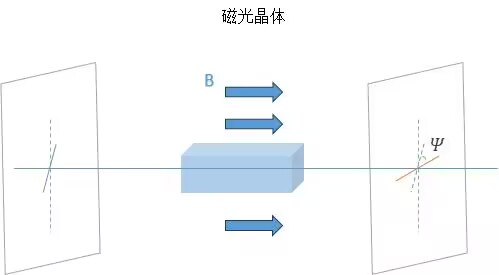
\includegraphics[width=0.45\textwidth]{磁致旋光.jpg} % 图片文件名和大小调整
    \caption{磁致旋光示意图} % 图片的标题
    \label{fig:磁致旋光示意图} % 图片的标签,用于引用
\end{figure}


在磁场的作用下,磁致旋光物质会产生
旋光性。如图\ref{fig:磁致旋光示意图}所示,当一束线线偏振光通过放
置于平行磁场中的磁致旋光物质时,光矢会
以主光轴为轴发生旋转。这种现象称为法拉
第效应或磁致旋光效应。磁场与旋转的角度
的关系为(详细推导见附录$C$。)
$$\Psi=VBl$$


其中,$V$ 是 Verder 常数,$B $是平行于线偏振光传输方向的磁场强度,
$l$ 是磁场与偏振光相互作用的有效长度。
\subsection{光自旋霍尔效应}
\begin{figure}[H] % h! 表示“尽可能在当前位置插入”
    \centering % 图片居中
    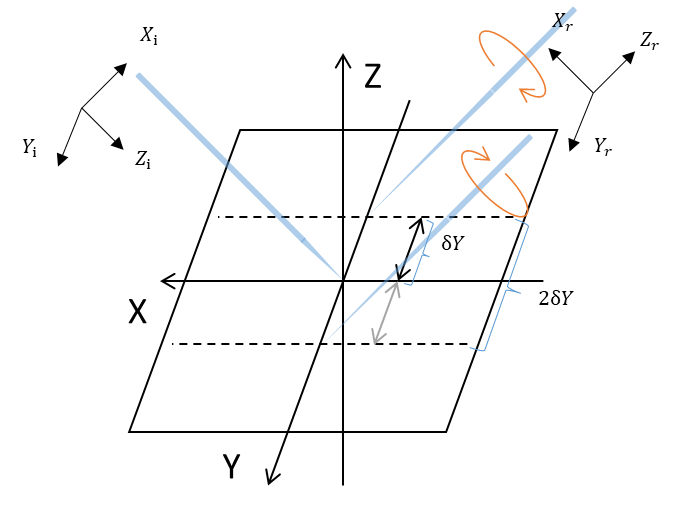
\includegraphics[width=0.5\textwidth]{光自旋霍尔效应示意图.png} % 图片文件名和大小调整
    \caption{光自旋霍尔效应图} % 图片的标题
    \label{fig:光自旋霍尔效应图} % 图片的标签,用于引用
\end{figure}

光自旋霍尔效应(Optical Spin Hall Effect, OSHE)是光子在介质界面反射和折射过程中,由于其自旋角动量的守恒性,导致的一个重要现象。具体而言,当光子入射到介质界面时,其中的左右旋圆偏振光(即自旋方向不同的光)会在反射和折射的过程中产生不同的位移。这种位移是为了维持整个系统的角动量守恒,表现为在垂直于入射光传播方向上,左右旋光在空间中的分离,如图 \ref{fig:光自旋霍尔效应图} 所示。

在实验中,我们可以观察到,当入射光通过一个具有非对称性或各向异性的介质(如某些光学材料或光学器件)时,具有不同自旋状态的光束在经过该界面时,分别会向y的方向偏移。


光自旋霍尔效应的实现涉及到光的自旋与轨道的耦合,同时也与介质的光学特性密切相关。

在本实验中主要还是以角谱理论解释光自旋霍尔效应

深入的证明过程及相关数学推导可见附录 $A$,其中详细阐述了光自旋霍尔效应的物理机制及实验观测方法。


\subsection{偏振相消干涉}
% 非对称量子弱测量是一种新型的测量方法,它通过在测量过程中引入一个非对称的测量基来减少测量误差。这种方法在量子力学中具有广泛的应用,特别是在量子计算和量子信息处理等领域。非对称量子弱测量可以有效地减少测量误差,提高测量精度,从而在量子计算和量子信息处理等领域具有广泛的应用前景。
\begin{figure}[H] % h! 表示“尽可能在当前位置插入”
    \centering % 图片居中
    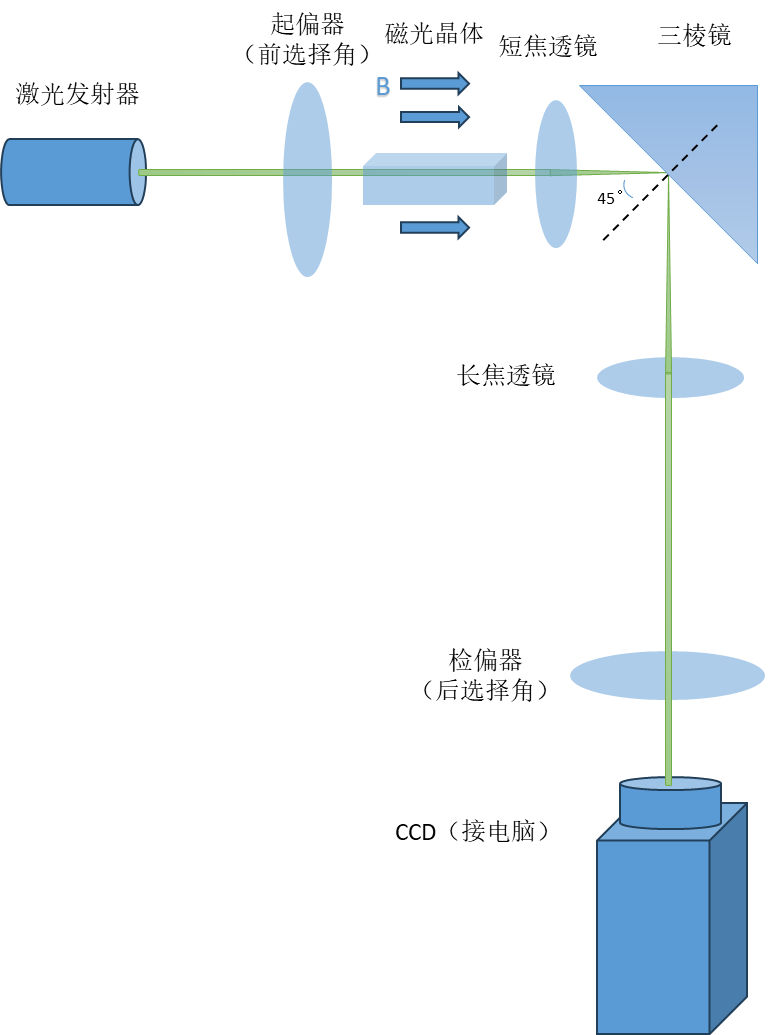
\includegraphics[width=0.6\textwidth]{实验装置图.png} % 图片文件名和大小调整
    \caption{实验装置示意图} % 图片的标题
    \label{fig:实验装置抽象图} % 图片的标签,用于引用
\end{figure}

偏振相消干涉是一种新型的测量技术,利用光的偏振态特性来实现高精度的测量。在这种测量方法中,我们通过引入非对称的测量基来降低测量过程中的误差,从而提高实验结果的可靠性。这一方法在多个物理领域中得到了应用,尤其是对于量子态的探测和操控有着重要意义。

如图 \ref{fig:实验装置抽象图} 所示,实验装置的示意图包括若干关键部件,依次为激光器发射器、起偏器(前选择角)、短焦透镜、三棱镜、长焦透镜、磁光晶体(外接螺线圈)、检偏器(后选择角)及 CCD(连接计算机以进行数据采集与处理)。

激光器发射出的光在经过高斯光起偏器后,光的偏振方向设置为水平偏振(H)。光经过磁光晶体时,其偏振方向会发生旋转,旋转的角度用 $\psi$ 表示,经过磁光晶体后的入射光可以表示为:

\begin{align*}
E^\psi(x,y) &= \cos\psi \, E^H(x,y) + \sin\psi \, E^V(x,y) \\
E^H &= G(x,y), \quad E^V = G(x,y)
\end{align*}

其中,$G(x,y)$ 是高斯光的振幅强度,上标 $H$ 和 $V$ 分别代表了水平和垂直偏振的光。

当光经过短焦透镜时,其会经历傅里叶变换,从位置空间转换到动量空间:

$$
E^\psi(k_x,k_y) = \mathcal{F}(E^\psi(x,y))
$$

在三棱镜处,发生光的自旋霍尔效应,使得反射光的表达式变为:

\begin{align*}
E^H_r(k_x,k_y) &= r_p G(k_x,k_y) e_H + r_p \delta y_r^H k_y G(k_x,k_y) e_V \\
E^V_r(k_x,k_y) &= -r_s \delta y_r^V k_y G(k_x,k_y) e_H + r_s G(k_x,k_y) e_V
\end{align*}

在上式中,下标 $r$ 表示反射光,$r_p$ 和 $r_s$ 分别为 $p$ 光和 $s$ 光的反射系数,$e_H$ 和 $e_V$ 为偏振基矢,而 $\delta y_r^H$ 和 $\delta y_r^V$ 则表示光在空间上的分离。详细的推导过程可以参考附录 B。

由于存在后选择角,我们只需关注反射光中与后选择角方向 $f$ 对齐的部分。一般情况下,方向 $f$ 对应于垂直偏振(V)方向。因此,我们在动量空间中,对光进行后选择角的投影,得到:

$$
E_r^{\psi \to f}(k_x,k_y) = r_p \left( \psi \eta G(k_x,k_y) + \delta y_r^H k_y G(k_x,k_y) \right)
$$

在这里,上标 $\psi \to f$ 表示对后选择角 $f$ 的投影。

随后,通过长焦透镜,光从动量空间转换回位置空间。我们可以通过分析光强在位置空间的分布,计算出光强质心的变化,给出如下关系:

$$
\Delta y = \frac{z}{R_0} \frac{2\psi\eta \delta y_{r}^{H}}{(1+\psi^2 \eta^2) \exp\left(k(\delta y_{r}^{H})^2/R_0\right) + \psi^2 \eta^2 - 1}
$$

在实验中,光的磁光旋转角 $\psi$ 通常约为 $10^{-4} \text{ rad}$,我们可以在 $\psi = 0$ 时对上述公式进行泰勒展开,并将 $\psi =Blv$代入,保留线性项后,得到本实验的理论公式:

\begin{equation}
\Delta y = \sigma B
\label{eq:理论公式}
\end{equation}

其中,$\sigma=1.326 m/T$(只考虑斜率的绝对值) ,具体含义和推导过程已在附录 C 中详细记录。

在实验过程中,光强质心偏移量 $\Delta y$ 可由 CCD 相机读取,从而得出所测得的磁场大小$B=\frac{\Delta y}{\sigma}$。









% \end{multicols}
% 插入图片


% \par % 换行,确保两张图片之间有间隔

% \begin{figure}[h!] % h! 表示“尽可能在当前位置插入”
%     \centering % 图片居中
%     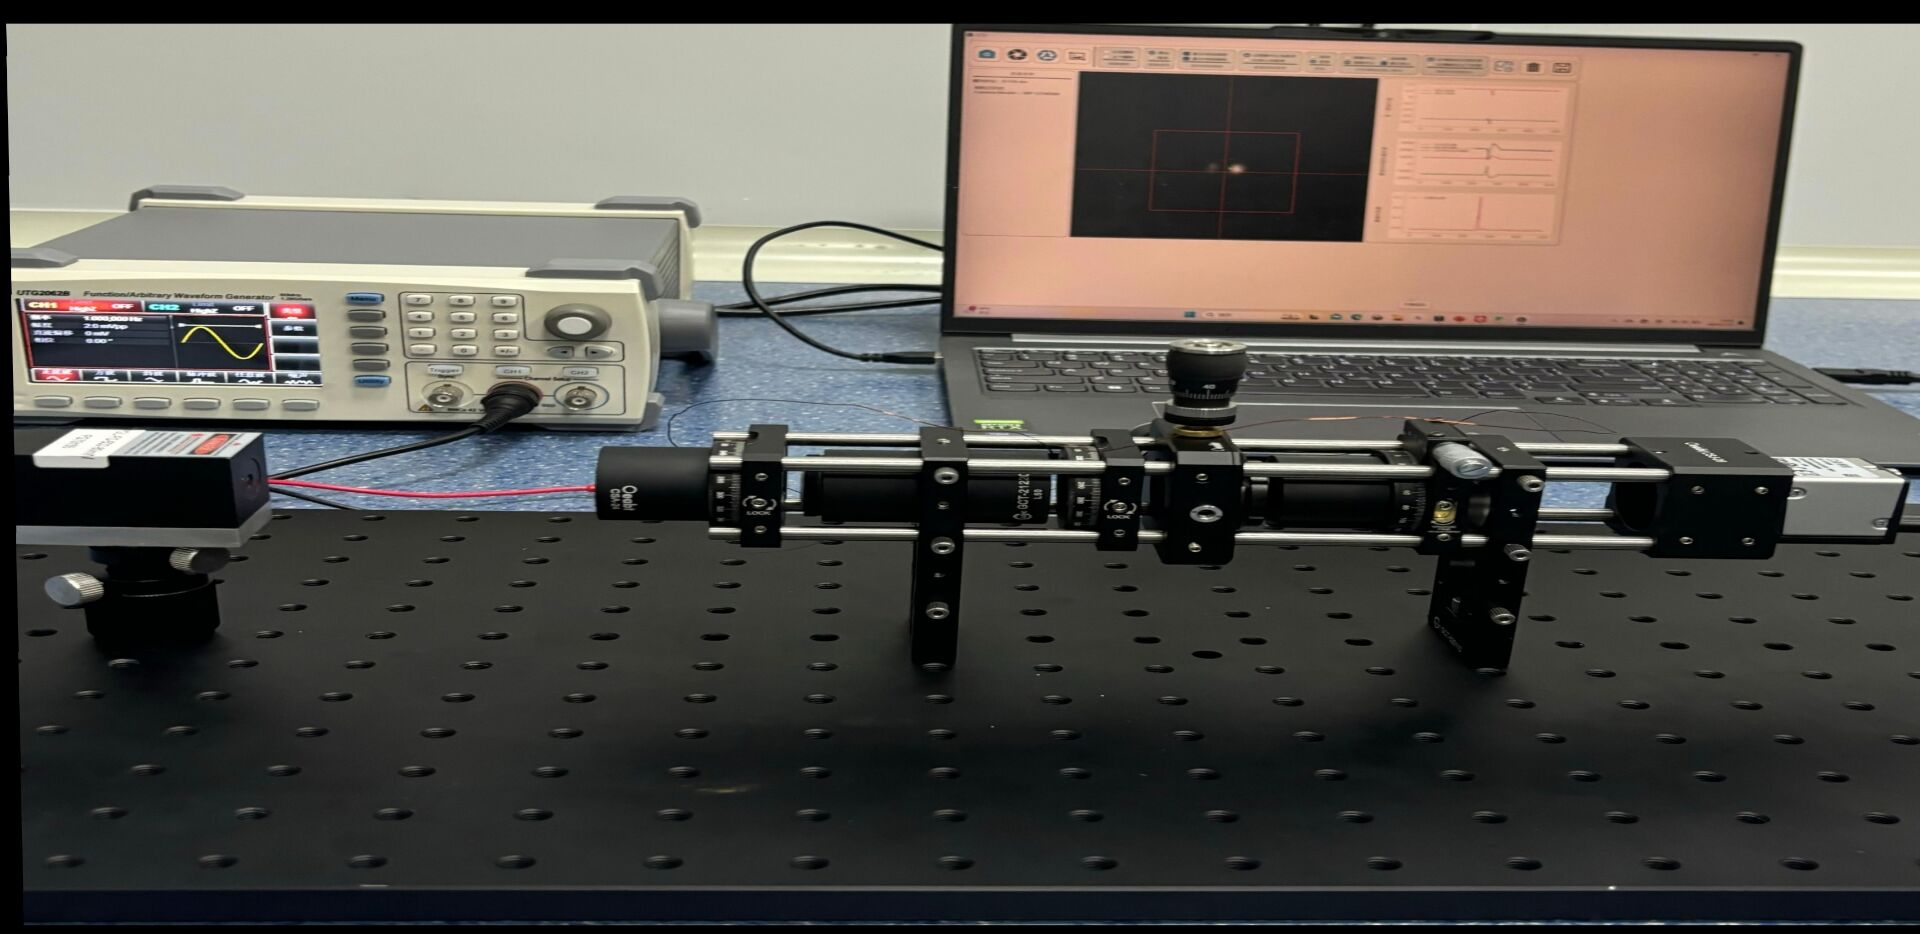
\includegraphics[width=0.75\textwidth]{实验装置实物图.jpg} % 图片文件名和大小调整
%     \caption{实验装置实物图} % 图片的标题
%     \label{fig:实验装置实物图} % 图片的标签,用于引用
% \end{figure}








% \begin{multicols}{2}
% \subsection{装置结构原理}
% \subsubsection{基本装置}

% 实验装置示意图如图\ref{fig:实验装置抽象图}所示,沿光路依次是激光器反射器、起偏器(前选择角)、磁光晶体(外接螺线圈)、短焦透镜、三棱镜、长焦透镜、检偏器(后选择角)、CCD(接电脑)。

% 理想情况下,前选择角(偏振器)与后选择角(偏振器)的偏振角应相互垂直。(实际情况下,只要满足消光条件即可)

% 微分元件()作用是使光分解成两个相互正交的偏振态,并使两分量在空间上分离一定距离,如图\ref{fig:对称光斑示意图}所示。

% CCD相机用于测量光心偏移量$C_x$

% \subsubsection{非对称偏振干涉磁场测量}
% 半导体激光器产生的532nm激光通过起偏器转化为线偏振光
% \begin{figure}[H] % h! 表示“尽可能在当前位置插入”
%     \centering % 图片居中
%     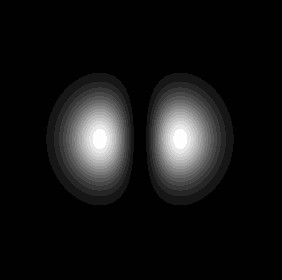
\includegraphics[width=0.25\textwidth ,trim=40pt 40pt 40pt 40pt, clip ]{对称光斑模拟图.jpg} % 图片文件名和大小调整
%     \caption{对称光斑模拟图} % 图片的标题
%     \label{fig:对称光斑模拟图} % 图片的标签,用于引用
% \end{figure}

% 不外加磁场时,激光器发出的高斯光束经过微分元件时,光的两个正交的偏振分量(分别设为水平光场和垂直光场)会相互分离(设两光心分离距离为$g$),通过调节微分元件的方向使得两分量的投影振幅相等,使得在到达CCD前,形成两个等大对称的光斑,如图\ref{fig:对称光斑模拟图}所示
% 此时,CCD上光强分布对称,总光心为0。


% % % \end{multicols}{}

% \begin{figure}[H] % h! 表示“尽可能在当前位置插入”
%     \centering % 图片居中
%     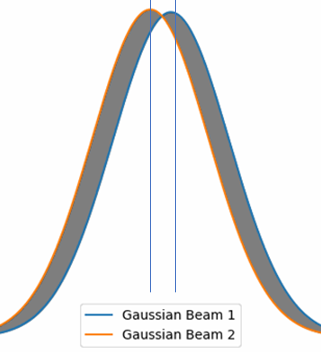
\includegraphics[width=0.2\textwidth ]{对称光斑示意图.png} % 图片文件名和大小调整
%     \caption{对称光斑示意图} % 图片的标题
%     \label{fig:对称光斑示意图} % 图片的标签,用于引用
% \end{figure}


% \begin{figure}[H]
%     \centering
%  \begin{minipage}{0.3\textwidth} % 设置 minipage 的宽度
%     \centering
%     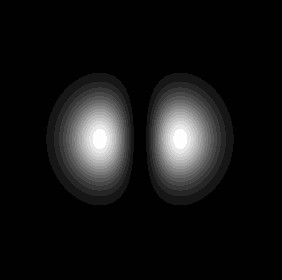
\includegraphics[width=\linewidth, trim=40pt 40pt 40pt 40pt, clip]{对称光斑模拟图.jpg} % 图片文件名和大小调整
%     \caption{对称光斑模拟图} % 图片的标题
%     \label{fig:对称光斑模拟图} % 图片的标签,用于引用
% \end{minipage}
% \hspace{0.15\textwidth} % 控制两个 minipage 之间的空白
%     \begin{minipage}{0.2\textwidth} % 设置 minipage 的宽度
%         \centering
%         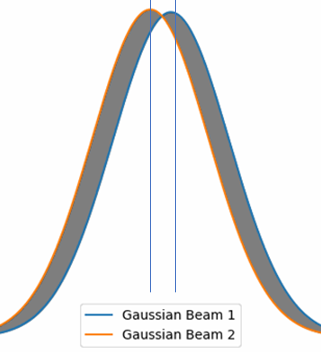
\includegraphics[width=\linewidth]{对称光斑示意图.png} % 图片文件名和大小调整
%         \caption{对称光斑示意图} % 图片的标题
%         \label{fig:对称光斑示意图} % 图片的标签,用于引用
%     \end{minipage}
% \end{figure}








% \begin{multicols}{2}
\section{实验现象}
在没有外加磁场的情况下,激光经过三棱镜时,会发生光自旋霍尔效应。此时,光束被分解为两个自旋相反的偏振态,并使这两分量在空间上分离一定距离。由于我们将入射光限定为 
H
H 光,因此两偏振态的振幅相等。通过后选择角,我们可以使得两自旋相反的光束在 CCD 上发生对称的相消干涉,如图 \ref{fig:对称光斑示意图} 所示。

两分量的投影振幅相等,使得在到达 CCD 之前形成两个等大且对称的光斑。在 CCD 上,光强的分布对称,总光心为 0。。
\begin{figure}[H] % h! 表示“尽可能在当前位置插入”
    \centering % 图片居中
    \begin{subfigure}{0.3\textwidth} % 设置子图宽度为0.45
        \centering
        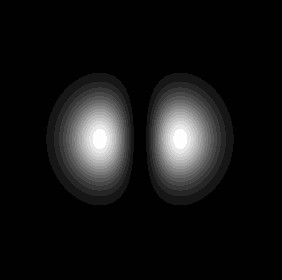
\includegraphics[width=\textwidth, trim=40pt 40pt 40pt 40pt, clip]{对称光斑模拟图.jpg} % 图片文件名和大小调整
        \caption{对称光斑模拟图} % 图片的标题
        \label{fig:对称光斑模拟图} % 图片的标签,用于引用
    \end{subfigure}
    \hspace{0.05\textwidth} % 设置两个图间的水平间距
    \begin{subfigure}{0.3\textwidth} % 设置子图宽度为0.45
        \centering
        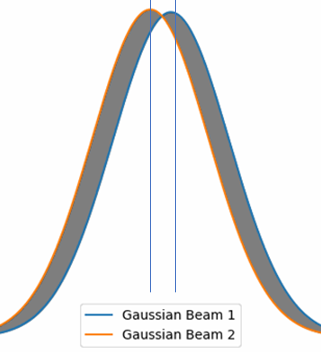
\includegraphics[width=\textwidth]{对称光斑示意图.png} % 图片文件名和大小调整
        \caption{对称光斑示意图} % 图片的标题
        \label{fig:对称光斑示意图} % 图片的标签,用于引用
    \end{subfigure}
    \caption{对称光斑相关图示} % 总标题
    \label{fig:对称光斑总图} % 总标签,用于引用
\end{figure}
当外加磁场时,激光经过磁光晶体,会因磁致旋光效应而发生变化。这里,偏振角的改变量记作 $\psi$,$B$ 为磁场强度,$V$为维尔德常量。在三棱镜处仍然发生光自旋霍尔效应,光束被分解为两个自旋相反的偏振态,并使两分量在空间上分离一定距离。然而,磁致旋光使得在三棱镜分解后的两个偏振态的振幅出现差别。通过后选择角,最终在 CCD 上发生非对称相消干涉,如图 \ref{fig:非对称光斑模拟图} 所示,导致 CCD 上光强的分布不对称。

通过计算前后两个光斑几何中心的总偏移量,可以得出磁场强度 
$B$从而实现对磁场的测量。





% \end{multicols}{}


\begin{figure}[H] % h! 表示“尽可能在当前位置插入”
    \centering % 图片居中
    \begin{subfigure}{0.3\textwidth} % 设置子图宽度为0.45
        \centering
        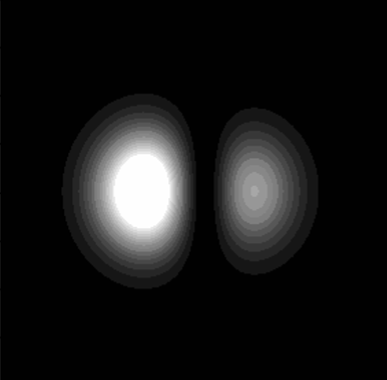
\includegraphics[width=\textwidth, trim=40pt 40pt 40pt 40pt, clip]{非对称光斑模拟图.png} % 图片文件名和大小调整
        \caption{非对称光斑模拟图} % 图片的标题
        \label{fig:非对称光斑模拟图} % 图片的标签,用于引用
    \end{subfigure}
    \hspace{0.05\textwidth} % 设置两个图间的水平间距
    \begin{subfigure}{0.3\textwidth} % 设置子图宽度为0.45
        \centering
        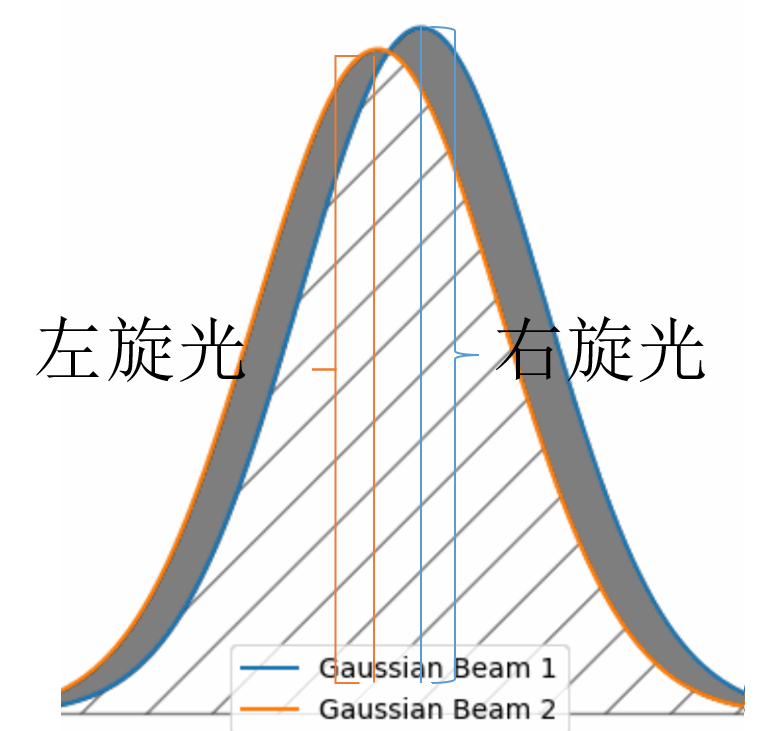
\includegraphics[width=\textwidth]{非对称光斑示意图.png} % 图片文件名和大小调整
        \caption{非对称光斑示意图} % 图片的标题
        \label{fig:非对称光斑示意图} % 图片的标签,用于引用
    \end{subfigure}
    \caption{非对称光斑相关图示} % 总标题
    \label{fig:非对称光斑总图} % 总标签,用于引用
\end{figure}


当我们施加交流磁场时,实验结果表明CCD相机上所采集到的图像质心平移量会呈现出周期性的交流振荡现象。这一现象的观察不仅证明了我们实验设置的有效性,还突显了通过此方法进行磁场测量的实时性与精准性。

具体而言,随着施加的交流磁场强度和频率的变化,CCD相机的输出信号也随之发生变化。质心平移量的周期性变化反映出磁场对探测物体的影响,这种动态响应为我们提供了关于磁场性质的重要信息。例如,质心的位移幅度和振荡频率可以帮助我们更好地理解交流磁场的分布特征及其对检测系统的影响。因此,通过对CCD相机捕获的图像进行精确分析,我们能够实时监测到施加磁场的变化,从而提升测量的准确性和灵敏度。
\begin{figure}[H]
    \centering
    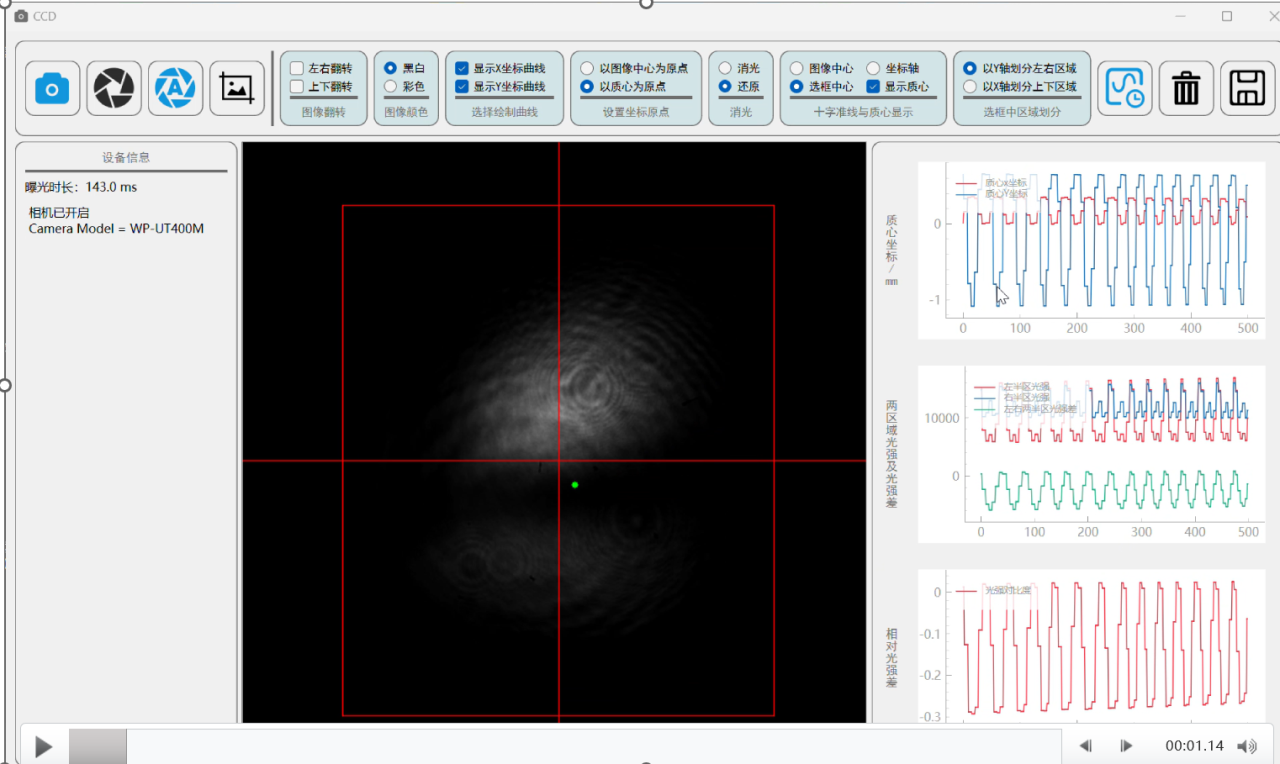
\includegraphics[width=0.6\textwidth]{交流信号图.png} % 图片文件名和大小调整
    \caption{CCD相机示意图} % 图片的标题
\end{figure}
% \begin{figure}[H]
%     \centering
%  \begin{minipage}{0.3\textwidth} % 设置 minipage 的宽度
%     \centering
%     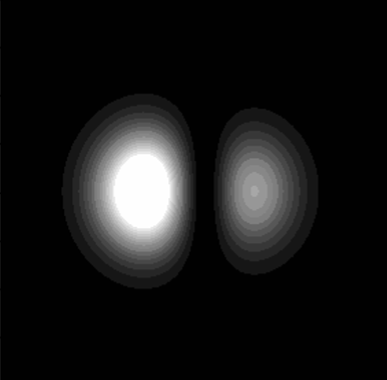
\includegraphics[width=\linewidth, trim=40pt 40pt 40pt 40pt, clip]{非对称光斑模拟图.png} % 图片文件名和大小调整
%     \caption{非对称光斑模拟图} % 图片的标题
%     \label{fig:非对称光斑模拟图} % 图片的标签,用于引用
% \end{minipage}
% \hspace{0.15\textwidth} % 控制两个 minipage 之间的空白
%     \begin{minipage}{0.2\textwidth} % 设置 minipage 的宽度
%         \centering
%         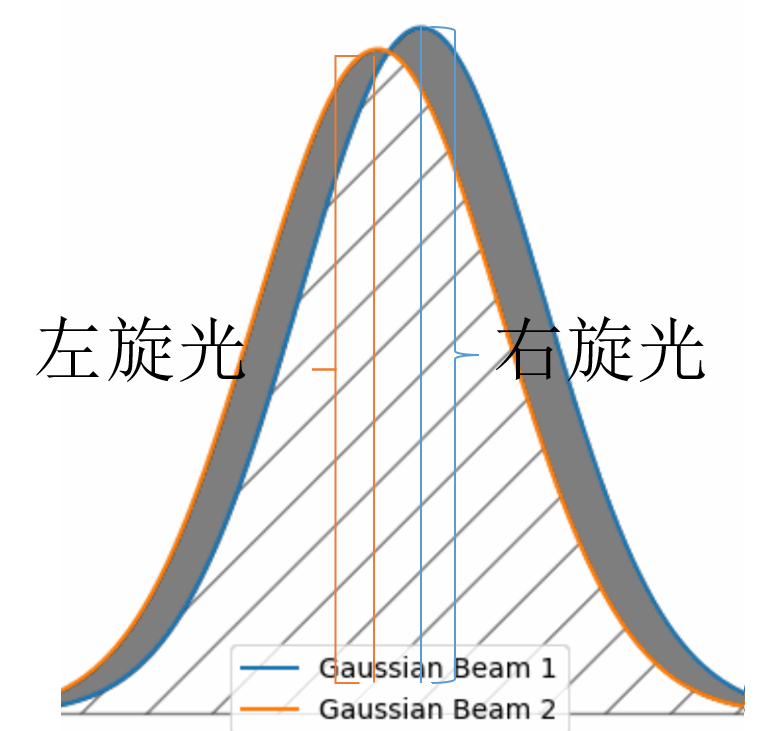
\includegraphics[width=\linewidth]{非对称光斑示意图.png} % 图片文件名和大小调整
%         \caption{非对称光斑示意图} % 图片的标题
%         \label{fig:非对称光斑示意图} % 图片的标签,用于引用
%     \end{minipage}
% \end{figure}
% \begin{multicols}{2}
% \subsubsection{光心偏移量和磁场强度理论公式}
% 如图\ref{fig:非对称偏振图}所示考虑磁光效应后,到达CCD上的水平和垂直光场光强分别为
% \begin{figure}[H] % h! 表示“尽可能在当前位置插入”
%     \centering % 图片居中
%     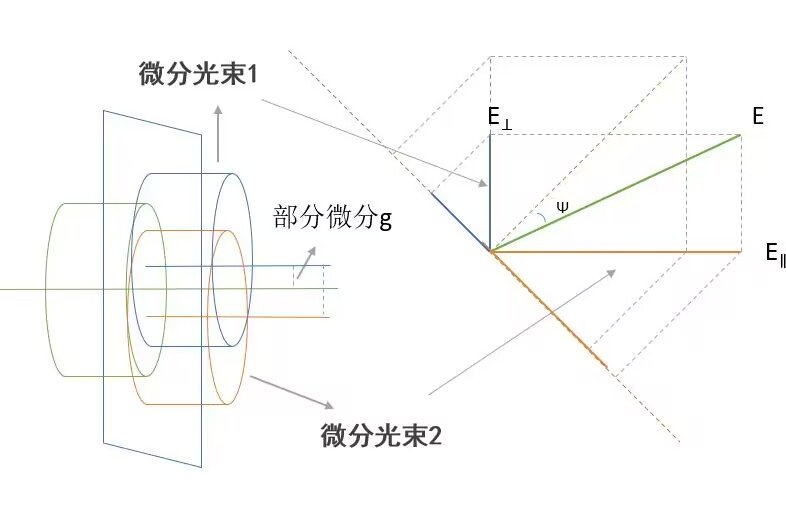
\includegraphics[width=0.4\textwidth]{非对称偏振图.jpg} % 图片文件名和大小调整
%     \caption{非对称偏振图} % 图片的标题
%     \label{fig:非对称偏振图} % 图片的标签,用于引用
% \end{figure}
% $$A_{\perp}=cos(\frac{\pi}{4}+\Psi)\frac{A_{0}}{\omega}exp(\frac{(x+0.5*g)^{2}}{\omega^{2}})$$
% $$A_{//}=cos(\frac{3\pi}{4}+\Psi)\frac{A_{0}}{\omega}exp(\frac{(x-0.5*g)^{2}}{\omega^{2}})$$
% 其中,$A_{0}$为激光束的振幅,$\omega$为光斑的半宽度,
% 故$A=A_{\perp}+A_{//}$
% 所以我们的光强分布
% $$I=A^*A$$
% 通过光心偏移量计算公式
% $$C_x=\frac{\iint_{-\infty}^{+\infty}\mathrm{x}Idxdy}{\iint_{-\infty}^{+\infty}Idxdy}$$
% 得到如下关系式
% $$C_x=\frac{gcos(\psi)Sin(\psi)}{1-e^{-\frac{g^2}{2\omega^2}}cos(\psi)}$$
% 考虑$\Psi$是一个小量上式可进一步简化为:
% $$C_x=\frac{2\omega^2lVB}g$$
% 即光心偏移量与磁场强度成正比,从而实现磁场测量。
% 所以我们最终得到
% $$B=\kappa C_x$$
% 其中$\kappa=\frac{g}{2\omega^2lV}$



















% \begin{figure}[h!]
%     \centering
%     \begin{minipage}{0.45\textwidth} % 设置 minipage 的宽度
%         \centering
%         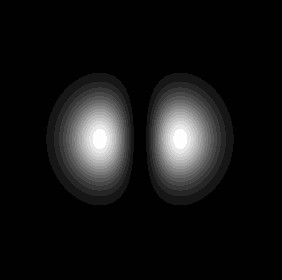
\includegraphics[width=\linewidth]{对称光斑模拟图.png} % 图片文件名和大小调整
%         \caption{对称光斑模拟图} % 图片的标题
%         \label{fig:对称光斑模拟图} % 图片的标签,用于引用
%     \end{minipage}
%     \hfill % 在两张图片之间插入空白
%     \begin{minipage}{0.45\textwidth} % 设置 minipage 的宽度
%         \centering
%         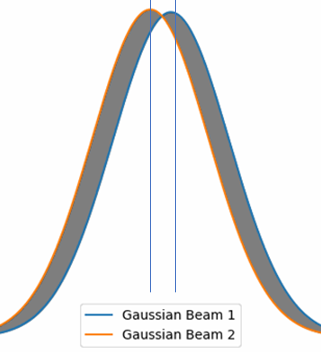
\includegraphics[width=\linewidth]{对称光斑示意图.png} % 图片文件名和大小调整
%         \caption{对称光斑示意图} % 图片的标题
%         \label{fig:对称光斑示意图} % 图片的标签,用于引用
%     \end{minipage}
% \end{figure}
\section{实验流程}

\begin{enumerate}

\item 按照图\ref{fig:实验装置抽象图}所示搭建实验仪器到光学平台上,选择合适的半导体激光光强,从左到右依次安装激光发射器、起偏器、磁光晶体(外接螺线圈)、短焦透镜、三棱镜、长焦透镜、检偏器、光屏,每安装一个仪器都使用孔径光阑验证光路准直且通过各元件中心。
\item 关闭环境灯光,在光屏上观察光斑形状及亮度,同时粗调起偏器、检偏器偏振角度,使光屏上上下的光斑大致出现大小一致,亮度相同。锁紧粗调螺钉。
\item 移走光屏,接入CCD,并且将CCD连接到电脑打开(依次打开镜头、自动曝光、自动计算,关闭x轴显示,将计算区域调至合适范围,打开光心显示),观察光斑图像。
\item 细调起偏器保证入射光沿$H$方向入射、检偏器偏振角度,使CCD中两个光斑形状相似,大小一致,亮度相同,并且使光心位置与图像几何中心(即选框中心)重合,在电脑上将其定为原点。
\item 使用鳄鱼夹连接螺线圈与信号发生器,打开信号发生器,输入直流信号(在信号发生器上表现为输入直流偏移量,将交流信号调节到远小于直流偏移量)。
\item 待图像稳定,观察并记录CCD中光心的偏移量。
\item 计算磁场强度
\end{enumerate}



\section{数据处理}
\subsection{微弱磁场的表征}
本实验旨在通过质心偏移量来计算磁场强度,为了验证我们实验方法的正确性,必须将测得的实验值与真实值进行对比。

在面对可分辨的磁场时,我们使用探针进行真实值的测量。然而,对于一些极微小的磁场,探针的测量能力受到限制,无法直接获取其真实值。为了有效表征这些微弱磁场,我们利用密绕螺线圈的特性,得知施加在螺线圈两端的电压与其产生的磁场强度之间存在正比例关系。因此,我们通过测量施加在螺线圈上的电压,并研究其与磁场强度之间的关系,以实现对微弱磁场的有效表征。


\begin{longtable}{p{2.5cm} p{3cm} p{3cm}} % 调整列宽
    \caption{直流偏移量与磁感应强度数据} \label{tab:拟合的磁感应强度} \\ 
    \toprule
    直流偏移量/V & 磁感应强度/mT & 拟合的磁感应强度/mT \\ 
    \midrule
    \endfirsthead % 表格第一页的表头
    \toprule
    直流偏移量/V & 磁感应强度/mT & 拟合的磁感应强度/mT \\ 
    \midrule
    \endhead % 表格后面的表头
    \bottomrule
    \endfoot % 表格的底部
    \endlastfoot % 最后一页的底部
    
    -11 & -0.86 & -0.858 \\
    -10 & -0.79 & -0.780 \\
    -9  & -0.71 & -0.702 \\
    -8  & -0.63 & -0.624 \\
    -7  & -0.53 & -0.546 \\
    -6  & -0.46 & -0.468 \\
    -5  & -0.39 & -0.390 \\
    -4  & -0.30 & -0.312 \\
    -3  & -0.22 & -0.234 \\
    -2  & null  & 0.000 \\
    -1  & null  & 0.000 \\
     0  & 0.00  & 0.000 \\
     1  & null  & 0.078 \\
     2  & null  & 0.156 \\
     3  & 0.22  & 0.234 \\
     4  & 0.30  & 0.312 \\
     5  & 0.39  & 0.390 \\
     6  & 0.46  & 0.468 \\
     7  & 0.53  & 0.546 \\
     8  & 0.63  & 0.624 \\
     9  & 0.71  & 0.702 \\
    10  & 0.79  & 0.780 \\
    11  & 0.86  & 0.858 \\ 
    \bottomrule
\end{longtable}
在实验中,我们获取的数据汇总如表\ref{tab:拟合的磁感应强度}所示。表中标记为“null”的部分表示无法利用探针进行磁场的实时测量,因此我们通过拟合的方法,推导出磁场强度与直流偏移量之间的关系,从而为微弱磁场的表征提供支持。

具体来说,为了确保实验的准确性和可靠性,我们预先通过探针探测密绕线圈的磁场分布,并得到施加在螺线圈上的电压(后文称为直流偏移量)与相应的磁场强度之间的良好线性关系。这样的关系促进了我们后续对微弱磁场的估算,解决了直接测量带来的困难。

% 在本实验中,我们通过密绕螺线圈制备均匀磁场,由于实验中的磁场强度较小无法直接使用探针进行测量,直同时接使用毕
% 奥萨法尔公式计算磁场强度较为困难,为此我们通过测定一定范围的磁场强度和施加在螺线圈上的电压(后文称为直流平移量)的关系,我们预先通过探针探测密绕线圈的磁场分布,得到磁场强度与施加在螺线圈上的电压(后文称为直流平移量)之间的关系,发现其及其良好的线性,

\begin{figure}[H] % h! 表示“尽可能在当前位置插入”
    \centering % 图片居中
    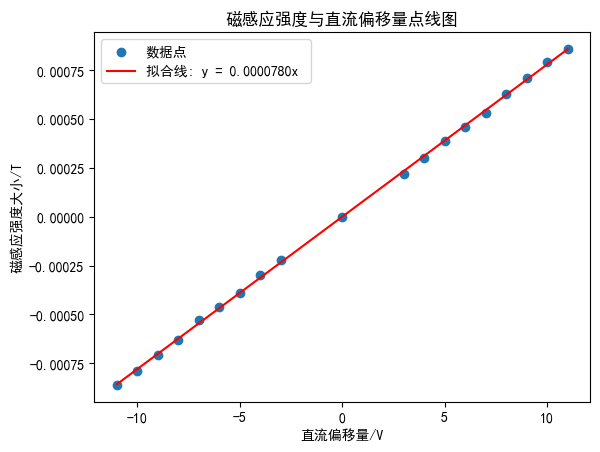
\includegraphics[width=0.6\textwidth]{磁场强度与直流偏移量的关系.png} % 图片文件名和大小调整
    \caption{磁场强度和直流平移量关系图} % 图片的标题
    \label{fig:磁场强度和直流平移量关系图} % 图片的标签,用于引用
\end{figure}

在数据拟合过程中,我们绘制了磁场强度与直流偏移量的关系图,如图\ref{fig:磁场强度和直流平移量关系图}所示。通过拟合,我们得到了高达$R^2 = 0.9997$的拟合优度,这说明实验数据之间的拟合效果非常良好,表明线性关系非常显著。由此,我们可以将直流偏移量(施加在螺线圈两端的电压,单位:V)代入此关系式,以近似计算磁场强度的实验值。

通过这种方法,我们成功解决了无法对极其微小磁场进行有效表征的问题,同时也增强了实验结果的可信性。此过程不仅验证了实验方法的正确性,更为后续研究奠定了基础。

\subsection{质心偏移量的测量}
在我们的实验中,我们注意到质心偏移量在不改变任何实验因素的情况下,会在一定范围内波动。为了减小测量误差,我们对每个磁场的质心偏移量进行了500次测量,并将结果以图表的形式展示,如图\ref{fig:质心偏移量的分布图}所示。

从图中可以看出,质心偏移量在实验过程中呈现出上下浮动的特征,这表明质心的偏移量变化是相对随机的。这种随机波动有效降低了弹簧应力对结果的影响,因为通常情况下,弹簧的应力会导致质心偏移量出现单向的偏移。通过进行多次测量,我们能够更好地确保最终得到的质心偏移量具有较高的有效性和可靠性。


\begin{figure}[H] % h! 表示“尽可能在当前位置插入”
    \centering % 图片居中
    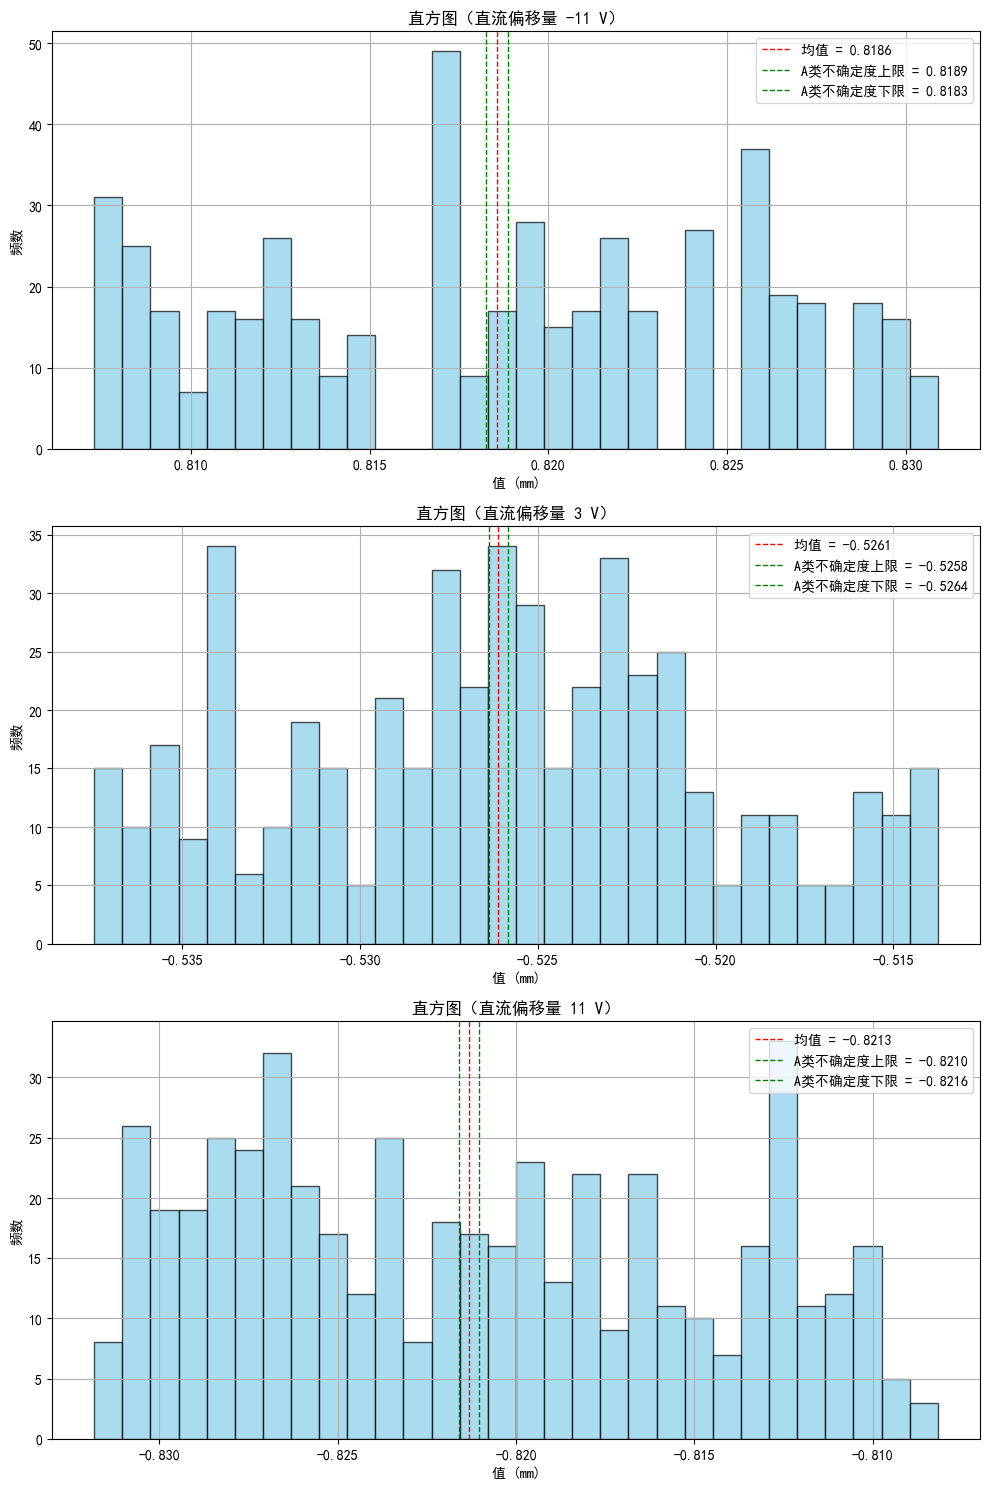
\includegraphics[width=0.6\textwidth]{质心偏移量的分布.png} % 图片文件名和大小调整
    \caption{质心偏移量的分布图} % 图片的标题
    \label{fig:质心偏移量的分布图} % 图片的标签,用于引用
\end{figure}
在CCD测量过程中,我们发现类别B的不确定度(取决于CCD相机的实际像素)远小于类别A的不确定度,因此我们将主要关注A类不确定度。最终的结果汇总如表\ref{tab:offset_uncertainty}所示,其中$V$表示施加在螺线圈两端的电压大小,作为直流偏移量的指标。这样的处理方式使得我们的结果更具科学性和准确性。


\begin{longtable}{p{2cm} p{4cm} p{3cm}} % 增大列宽
    \caption{质心偏移量} \label{tab:offset_uncertainty} \\ 
    \toprule
    直流偏移量/V & 均值 ($\mu$m) & $u_a$ ($\mu$m) \\
    \midrule
    \endfirsthead % 表格的第一页头部
    
    \toprule
    直流偏移量/V & 均值 ($\mu$m) & $u_a$ ($\mu$m) \\
    \midrule
    \endhead % 表格的后续页头部
    
    \bottomrule
    \endfoot % 表格底部,一般在最后一页
    
    \endlastfoot % 表格最后一页底部
    -11 & 818.6 & 0.3054 \\
    -10 & 843.8 & 0.9614 \\
    -9  & 651.5 & 0.1953 \\
    -8  & 636.0 & 0.0234 \\
    -7  & 641.8 & 0.1932 \\
    -6  & 690.4 & 0.8260 \\
    -5  & 857.1 & 0.6035 \\
    -4  & 541.7 & 0.2900 \\
    -3  & 491.5 & 0.5294 \\
    -2  & 276.1 & 0.7611 \\
    -1  & 157.0 & 0.5124 \\
    0   & 0.0   & 0.0 \\
    1   & -205.4 & 0.1074 \\
    2   & -391.9 & 0.2167 \\
    3   & -526.1 & 0.2701 \\
    4   & -577.4 & 0.8692 \\
    5   & -809.5 & 0.2715 \\
    6   & -897.7 & 0.3473 \\
    7   & -1063.4 & 0.2431 \\
    8   & -1078.7 & 0.1585 \\
    9   & -1143.3 & 0.4265 \\
    10  & -927.8 & 0.0670 \\
    11  & -821.3 & 0.2898 \\
    \bottomrule
\end{longtable}
\subsection{实验结果}
我们通过直流偏移量(单位:V)标定螺线圈产生的磁场,通过CCD相机读取光强分布的光心偏移量,将实验结果与理论测量的结果作对比得到图如下:

\begin{figure}[H] % h! 表示“尽可能在当前位置插入”
    \centering % 图片居中
    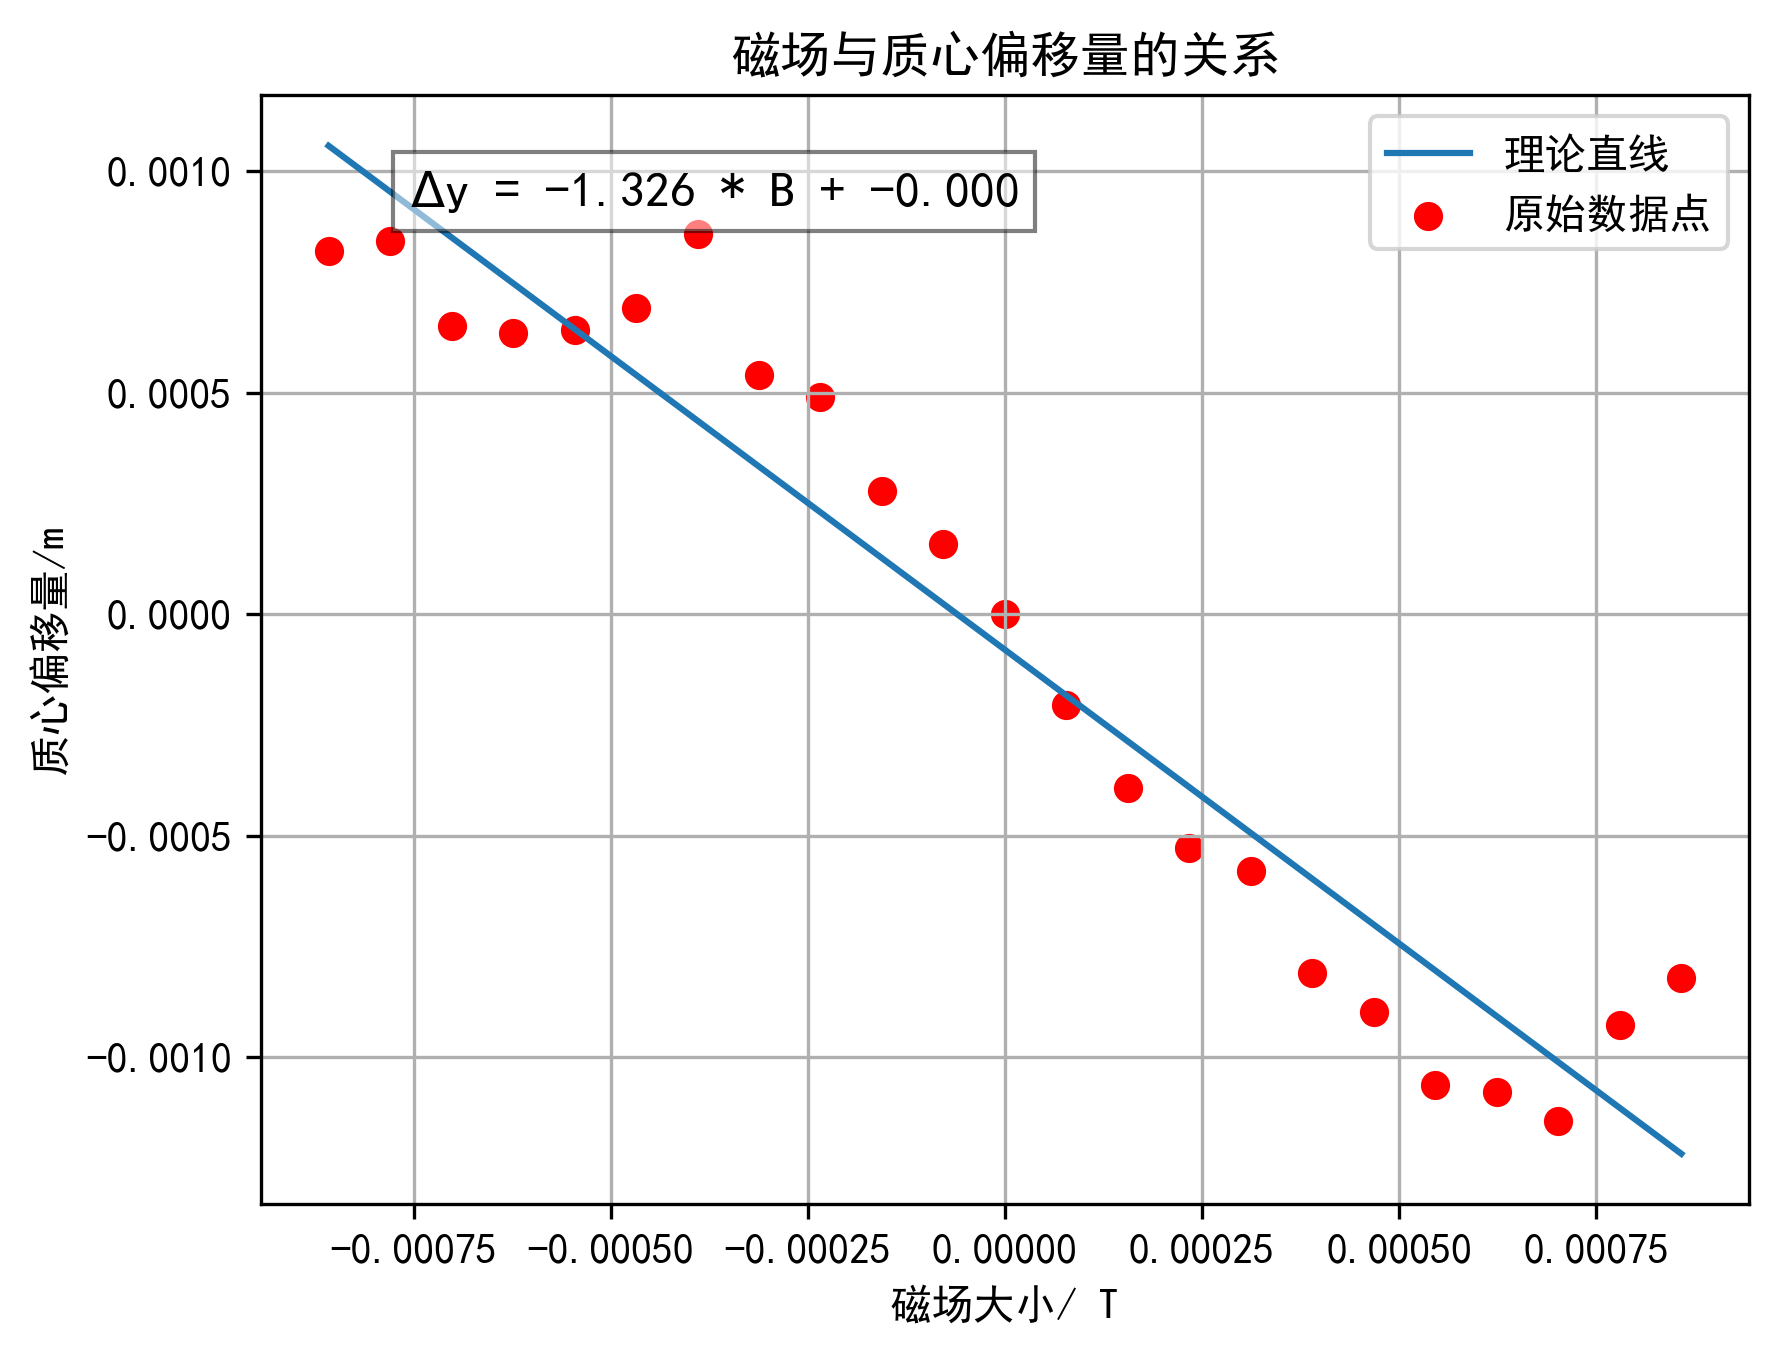
\includegraphics[width=0.6\textwidth]{磁场与质心偏移量的关系.png} % 图片文件名和大小调整
    \caption{光心偏移量(x)随磁场强度变化的实验关系图} % 图片的标题
    \label{fig:有效区间} % 图片的标签,用于引用
\end{figure}
在一定范围内,实验数据与理论值之间的相对误差不超过5\%,因此实验结果具有较高的准确性和可靠性。

\section{误差分析}
\subsection{理论公式近似的有效区间}

根据一般的质心偏移量与磁场强度之间的关系,满足下式:

\[
\Delta y = \frac{z}{R_0} \frac{2\psi\eta \delta y_{r}^{H}}{(1+\psi^2 \eta^2) \exp\left(k(\delta y_{r}^{H})^2/R_0\right) + \psi^2 \eta^2 - 1}
\]

由于该式为非线性关系,因此无法直接反解出磁场强度与质心偏移量之间的关系。

为此,我们采用线性化处理,将质心偏移量与磁场强度之间的关系近似为线性关系,从而得出磁场强度与质心偏移量之间的关系:

\[
\Delta y = \sigma B
\]

其中,\(\sigma = 1.326\)(仅考虑绝对值的比例关系)。

由此,我们可以表示磁场强度与质心偏移量之间的关系为:

\[
B = \frac{\Delta y}{\sigma}
\]

接下来,我们需要对该近似关系的有效范围进行说明。由于我们无法反解出一般情况下的磁场强度与光心偏移量之间的关系,因此我们通过对质心偏移量与磁场强度的关系进行近似求解,以确定其有效范围。

设定线性关系为:

\[
\Delta y^* = \sigma B
\]

我们可以进一步分析误差:

\[
\text{误差} = \frac{|\Delta y^* - \Delta y|}{\Delta y}<5\%
\]

通过数值方法,求解满足上述条件的磁场强度:
\begin{figure}[H] % h! 表示“尽可能在当前位置插入”
    \centering % 图片居中
    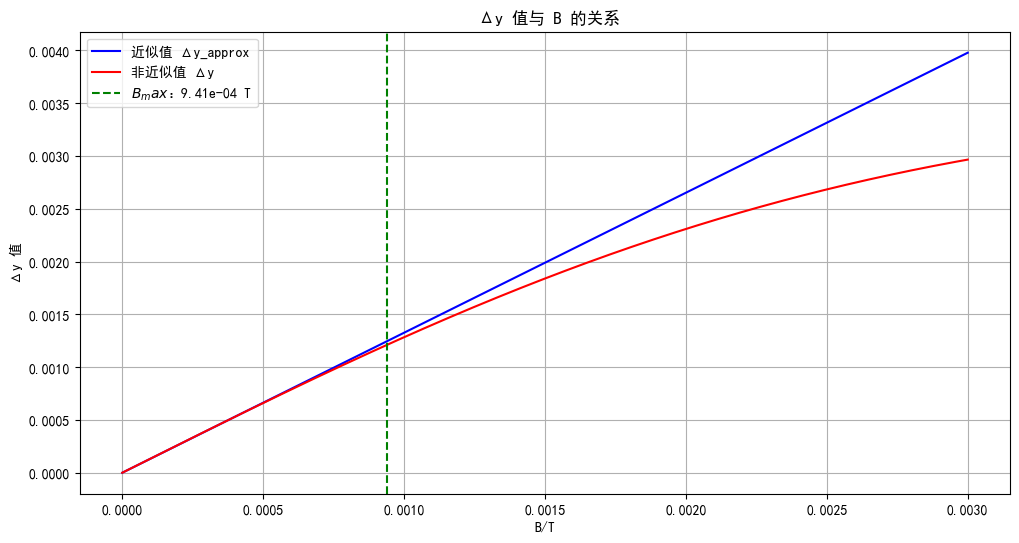
\includegraphics[width=0.7\textwidth]{近似区间.png} % 图片文件名和大小调整
    \caption{光心偏移量(x)随磁场强度变化的理论关系图} % 图片的标题
    \label{fig:有效区间} % 图片的标签,用于引用
\end{figure}


由图可知我们的磁场在$941\mu T$以内该线性近似是有效的。
% \end{multicols}

% 由于通过光心偏移量计算磁场强度的公式是一个近似公式,因此我们要求未近似的反解公式与近似公式之间的相对误差不超过百分之五。基于这一条件,我们得到结果的有效范围,如下图所示。
% \begin{figure}[H] % h! 表示“尽可能在当前位置插入”
%     \centering % 图片居中
%     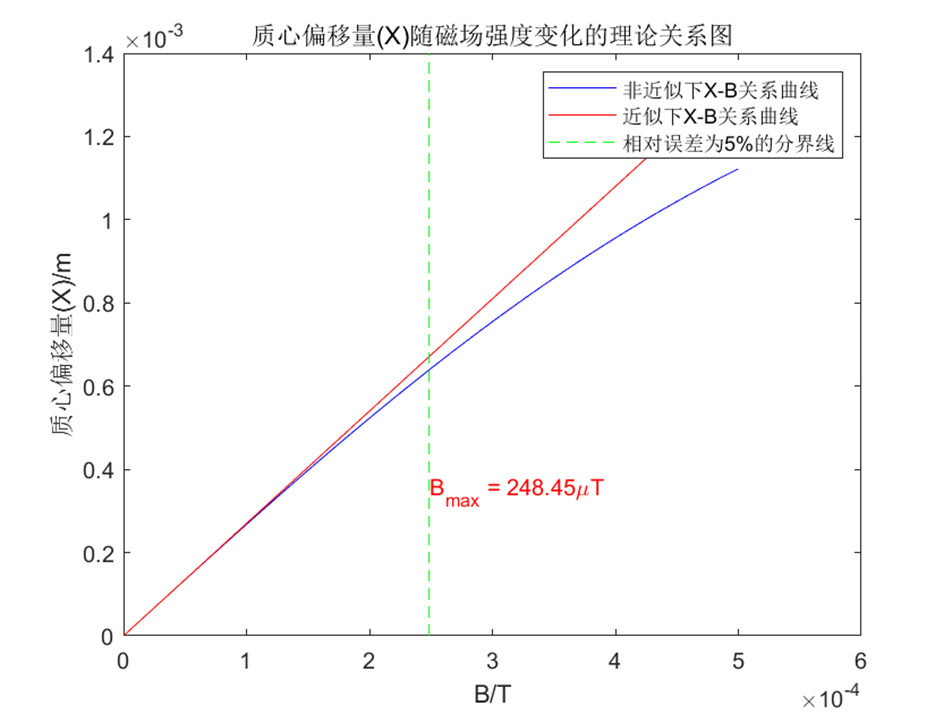
\includegraphics[width=0.5\textwidth]{有效范围.png} % 图片文件名和大小调整
%     \caption{光心偏移量(x)随磁场强度变化的理论关系图} % 图片的标题
%     \label{fig:有效区间} % 图片的标签,用于引用
% \end{figure}
% \end{multicols}

% \begin{multicols}{2}

% \subsection{不确定度的分析}
% 我们通过施加测试磁场得到数据如下表
% \begin{table}[H]
%     \hspace{-1cm} % 根据需要调整负的水平间距
%     \begin{tabular}{ccccccc}
%         \toprule
%         $C_X$/$10^{-5}$m & 1.1 & 2.2 & 3.5 & 4.5 & 5.5 & 6.6 \\
%         \midrule
%         B/$10^{-6}$T & 4.1 & 8.40 & 1.25 & 1.68 & 2.09 & 2.51 \\
%         \midrule
%         $E_N$ & 9.1\% & 4.5\% & 2.8\% & 2.2\% & 1.8\% & 1.5\% \\
%         \bottomrule
%     \end{tabular}
%     \caption{测试磁场数据}
%     \label{tab:测试磁场数据}
% \end{table}
% 绘制曲线如下
% \begin{figure}[H] % h! 表示“尽可能在当前位置插入”
%     \centering % 图片居中
%     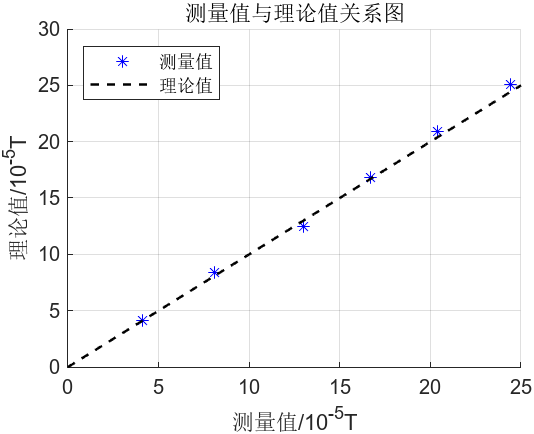
\includegraphics[width=0.5\textwidth]{实验数据图.png} % 图片文件名和大小调整
%     \caption{测量值与理论值关系图} % 图片的标题
%     \label{fig:实验数据} % 图片的标签,用于引用
% \end{figure}
% 由图可以理论值和测量值近似在过原点斜率为$1$的直线上

% 由误差传递公式可以知道,相对不确定度
% \[
% E_N = \sqrt{\left(\frac{C_x}{u_{c_x}}\right)^2 + \left(\frac{L}{u_L}\right)^2}.
% \]
% \noindent
% \(\frac{1}{L}u_L\) 很小,基本可以忽略不计,误差基本来自于 \(C_x\),根据 \(C_x\) 的值,可以大致估算出在多次测量的理想情况下的相对不确定度(\(u_{c_x} = 10^{-6} \text{m}\))。

% 从表格中可以看出,因为测量$C_x$精度的限制,当 B$<8.4*10^{-6}T$时,测量带来的不确定度将大于 8\%,而当 B 增大时,测量带来的不确定度将减少,直到线性拟合带来的误差占误差的主要部分。因此,我们可以初步估计我们的测量范围为 -2.48*10$^{- 4}($T)<B$< 2. 48* 10^- 4($T) ,测 量 精 度 为$0. 37* 10^{- 6}($T),考虑要在误差允许范围内(<5\%),我们的测定范围(即在误差允许范围内的磁场强度)为$8*10^{-6}$(T)到 $2.48*10^{-4}$(T)(包含此范围的负值)。









% \section{实验仪器}
% 半导体激光器、偏振片、CCD相机、磁光晶体、三棱镜、通电螺线管

% 具体实验仪器规格见附录
\subsection{磁化效应的讨论}
为了避免磁光晶体在施加磁场的过程中,由于其对外场的效应,会产生一定的磁化效应,从而导致磁光效应的磁场与螺线圈实际产生的磁场之间存在一定的偏差,因此我们需要对磁化效应进行讨论。

验证方法就是在在有无磁光晶体的环境测量磁场强度是否出现明显的变化,通过控制变量(保持在直流偏移量相同的条件下),我们的得到实验结果如下:
\begin{figure}[H] % h! 表示“尽可能在当前位置插入”
    \centering % 图片居中
    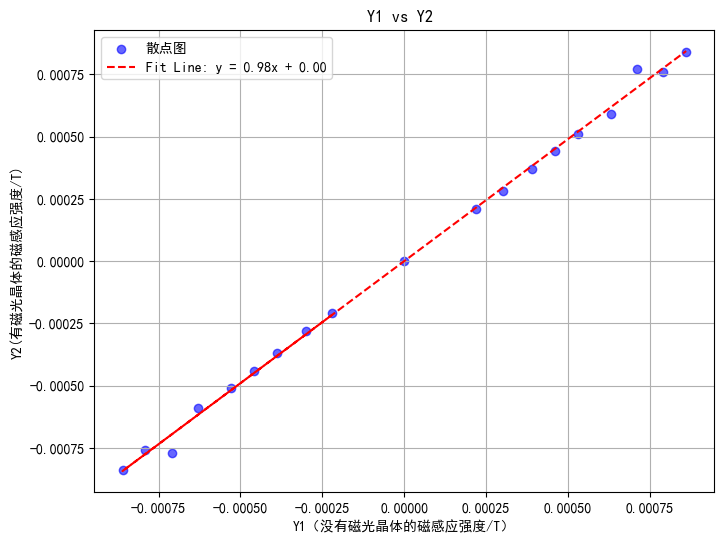
\includegraphics[width=0.6\textwidth]{有无磁光晶体的对比.png} % 图片文件名和大小调整
    \caption{有无磁光晶体时磁场强度的分布关系图} % 图片的标题
    \label{fig:有无磁光晶体时磁场强度的分布关系图} % 图片的标签,用于引用
\end{figure}
由图可知,在施加直流偏移量相同的情况下,磁光晶体对磁场强度的影响微乎其微,其平均相对误差为$4.91\%$,我们测定的磁场通常在几十微特左右,考虑相对误差之后,其影响至多不超过$0.5\mu T$,因此我们可认为磁光晶体对实验结果影响微乎其微,可以忽略不计。

\subsection{不确定度分析}

在本实验中,我们从 A 类不确定度的角度对磁场的测量不确定度进行了详细分析。首先,磁场的 A 类不确定度主要来源于质心偏移量的读取。为了获得更为准确的测量结果,我们进行了 500 次独立的测量,并对这些结果进行了统计分析。通过应用误差传递公式,我们可以估算出磁场测量的不确定度,公式表示为:

\[
\Delta y = \sigma B,
\]

其中,$\Delta y$ 代表磁场测量的不确定度,$\sigma=1.326$ 为一常数,而 $B$ 则是实际所测量的磁场强度。经过计算,我们发现质心偏移所导致的磁场不确定度的量级约为 $10^{-7} \text{ T}$,这一结果为后续分析提供了基础数据。

其次,除了质心偏移引起的不确定度外,我们还需考虑磁化效应所带来的不确定度。磁化效应的测量误差同样也在 $10^{-7} \text{ T}$ 的量级范围内。因此,质心偏移和磁化效应两者的不确定度相对接近,不能在最终的不确定度分析中被忽略。

综合上述分析,基于以上两种主要来源的误差,我们可以合理地认为,本实验测得的磁场的不确定度量级为 $10^{-7} \text{ T}$。换句话说,我们的实验精度达到了 $10^{-6} \text{ T}$,这使得我们在实验中能够获得较高的测量可靠性。

通过对这两个来源的不确定度进行综合评估,我们不仅可以深入理解实验结果的准确性,还能够为今后的研究提供重要的参考依据。这种严谨的分析方法为进一步优化实验设计和改进测量系统提供了坚实的基础。














\section{注意事项}
\begin{enumerate}
\item 为避免自然光对实验结果产生干扰,实验应该在无光或弱光环境下进行。
\item 实验全程不可用手触碰元件光学表面(包括透镜、偏振片、磁光晶体、微分元件、CCD光学界面等),避免损坏元件。
\item 不可对磁光晶体施加过大压力,以避免光弹效应干扰实验现象
\item 半导体激光器不完全稳定。
\end{enumerate}

% \section{实验误差原因分析}
% \begin{enumerate}
%     \item 激光器需用风扇散热,会导致测量结果在较小范围内存在震荡,影响测量结果。
% \end{enumerate}
\section{应用前景}
\begin{enumerate}
    \item 高精度磁场测量:现阶段磁光晶体维尔德常量最高可达600,可使磁场测量精度达到T。这将有助于深入了解材料的磁性特性和变化规律。
\item 动态研究:实时显示测量结果可以使研究人员观测瞬态磁现象和快速变化的磁场分布,如磁性材料的磁化过程、磁通量涡旋的动态行为等
\item 工业应用:①非接触式测量:由于不需要\cite{郭永康1992光学教程}电接触,磁光晶体测量方法特别适用于需要非入侵测量的场合,例如高温、高压环境中的磁场监测已经可燃性气体环境中的磁场②在线监控与质量控制:在生产过程中实时监控磁场,有助于维护设备的最佳运行状态,并及时发现和纠正潜在故障,提高生产效率
\item 磁性材料检测与定量分析:在医疗器械和药物开发中,精确测量磁性材料的磁场强度将有助于优化材料性能,从而提高器械和药物的质量。
\item 磁共振成像(MRI):高精度和实时检测能力将进一步提升MRI设备的性能,改善图像质量,同时降低操作难度和成本。
\end{enumerate}
\section{成员分工}
在本次实验中,团队成员相互协作、共同完成实验比赛。
成员1进行实验操作与实验数据采集。成员2进行实验原理与公式推导。成员3进行实验公式验证与不确定度分析。成员4进行课件制作和视频剪辑。成员5负责汇总与视频拍摄。

% \end{multicols}
\bibliographystyle{unsrt} % 参考文献样式为序号
\bibliography{ref} % 指定 .bib 文件名














































\newpage
\appendixformat
\section{光自旋霍尔效应}
\subsection{基本思路}
\begin{itemize}

    \item  建立中心波矢坐标系 $(\mathrm{x}_\alpha, \mathrm{y}_\alpha, \mathrm{z}_\alpha)$ 和任意波矢坐标系 $(\mathrm{X}_{\alpha}, \mathrm{Y}_{\alpha}, \mathrm{Z}_{\alpha})$,其中 $\alpha = i, r$ 表示入射、反射。

    \item 将入射电场由中心波矢坐标 $(x_i, y_i, z_i)$ 通过坐标旋转变换到任意波矢坐标 $(X_i, Y_i, Z_i)$。

    \item  由该任意波矢的入射坐标,通过反射变换到任意波矢的反射坐标 $(X_r, Y_r, Z_r)$ 。对于单个角谱分量而言,其严格遵循反射定律。

    \item  由该任意波矢的反射坐标同样经过坐标旋转,重新变回到中心波矢的反射坐标 $(x_r, y_r, z_r)$。

\end{itemize}

\subsection{反射矩阵的推导}
任意线偏振光可以看成是同频率的左旋与右旋圆偏振光叠加,根据琼
斯矩阵,对于水平(H)和垂直(V)偏振光,其角谱表达式:


$$\tilde{E}_{\alpha}^{H}=\frac{1}{\sqrt{2}}(\tilde{E}_{\alpha+}+\tilde{E}_{\alpha-})$$
$$\tilde{E}_{\alpha}^{V}=\frac{1}{\sqrt{2}}i(\tilde{E}_{\alpha-}-\tilde{E}_{\alpha+})$$

$“_+”与“_-”分别代表$
左旋与右旋圆偏振

入射光束为高斯形且具有有限的角谱宽度:

$$\tilde{E} _{i}( k_{ix}, k_{iy}) = \frac {w_{0}}{\sqrt {2\pi }}\exp \left \lceil - \frac {w_{0}^{2}( k_{ix}^{2}+ k_{iy}^{2}) }4\right \rceil$$

$w_0$为束腰半径,$k_{ix}$,$k_{iy}$表示入射波矢在$x$和$y$方向上面的分量。

\begin{enumerate}
    \item 绕$y$轴旋转$\theta_{i}$角,把入射场的中心波矢坐标系$( x_i,y_i,z_i)$变换到基点
    坐标系 $(x,y,z)$。(绕y轴旋转$\theta_{i}$角,$\theta_{i}$为入射角)

    \begin{align*}&\text{表述为:}\quad\tilde{E}_{_{xyz}}=m_{_{x_iy_iz_i\to xyz}}\tilde{E}_{_{x_iy_iz_i}}\\\\&\text{变换矩阵为:}\quad m_{_{x_iy_iz_i\to xyz}}=\begin{pmatrix}\cos\theta_i&0&-\sin\theta_i\\0&1&0\\\sin\theta_i&0&\cos\theta_i\end{pmatrix}\end{align*}
    \item 以 $z$ 轴为旋转轴,通过转旋角度 $\frac{k_{iy}}{k_0 \sin{\theta_i}}$

    \begin{alignat*}{1}
        \text{变换矩阵为:} m_{xyz \to XYZ} = \begin{pmatrix}
            1 & \frac{k_{iy}}{k_{0} \sin \theta_{i}} & 0 \\
            -\frac{k_{iy}}{k_{0} \sin \theta_{i}} & 1 & 0 \\
            0 & 0 & 1
        \end{pmatrix}
    \end{alignat*}
    
    其中 $k_0$ 代表真空中的波数。
    \item 再以 y 轴为旋转轴,通过旋转角度 -$\theta_{i}$ ,将电场由基点坐标变到任意波矢的入射坐标$(X_i,Y_i,Z_i)$。
    $$\text{变换矩阵为:}m_{_{XYZ\to X_i,Y_iZ_i}}=\begin{pmatrix}\cos\theta_i&0&\sin\theta_i\\0&1&0\\-\sin\theta_i&0&\cos\theta_i\end{pmatrix}$$


综合得到电场由坐标 (x$,y_i,z_i)$变换到坐示$( X_{i}, Y_{i}, Z_{i})$ 的整个过程。

$$\tilde{E}_{x_iy_iz_i}=M_{x_iy_iz_i\to X_iY_iZ_i}\tilde{E}_{X_iY_iZ_i}$$

$$M_{x_iy_iz_i\to X_iY_iZ_i}=m_{XYZ\to X_iY_iZ_i}m_{xyz\to XYZ}m_{x_iy_iz_i\to xyz}$$

得到如下关系式:
$$M_{x_i,y_iz_i\to X_iY_iZ_i}=\begin{pmatrix}1&k_{iy}\cot\theta_i/k_0&0\\-k_{iy}\cot\theta_i/k_0&1&k_{iy}/k_0\\0&-k_{iy}/k_0&1\end{pmatrix}$$

以上考虑的都是三维矩阵,实际上由散度方程:$\tilde{E}_{rz}k_{rz}=-(\tilde{E}_{rx}k_{rx}+\tilde{E}_{ry}k_{ry})$可以求得其 z分量
在接下来的计算中可以只考虑二维的矩阵

$$\tilde{E}_{X_rY_rZ_r}=r_{p,s}\tilde{E}_{X_iY_iZ_i}$$

 $\mathbf{r}_{\mathrm{p,s}}$为菲涅尔反射系数

 \item 根据菲涅尔反射定律求出反射场:

 \[
 \tilde{E}_{X_r Y_r Z_r} = r_{p,s} \tilde{E}_{X_i Y_i Z_i} \quad \text{其中 } r_{p,s} \text{ 为菲涅尔反射系数}
 \]
\item 最后,在把坐标$(\mathrm X_r,\mathrm Y_r,\mathrm Z_r)$变回到中心波矢的反射坐标$(x_r,y_r,z_r)$。其变换的过程为1—3的逆向过程
\begin{itemize}
    \item 绕 $y$ 轴旋转 $-(\pi - \theta_i)$ 将 $(X_r, Y_r, Z_r)$ 坐标系旋转到基点坐标 $(X, Y, Z)$。

    \[
    M_{X_r Y_r Z_r \to XYZ} = \begin{bmatrix}
        \cos\left[-\left(\pi - \theta_i\right)\right] & 0 & \sin\left[-\left(\pi - \theta_i\right)\right] \\\\
        0 & 1 & 0 \\\\
        -\sin\left[-\left(\pi - \theta_i\right)\right] & 0 & \cos\left[-\left(\pi - \theta_i\right)\right]
    \end{bmatrix}
    \]
    \item$ \text{绕 } z \text{ 轴旋转 } -\frac{k_{iy}}{k_0 \sin{\theta_i}} \text{ 角,将坐标 } (X,Y,Z) \text{ 变回到基点坐标系 } (x,y,z)。$
    \[
        M_{XYZ \to xyz} = \begin{bmatrix}
            1 & -\frac{k_{iy}}{k_0 \sin{\theta_i}} & 0 \\\\
            \frac{k_{iy}}{k_0 \sin{\theta_i}} & 1 & 0 \\\\
            0 & 0 & 1
        \end{bmatrix}
        \]
    \item 绕$ y $ 轴旋转
    $( \pi  -  \theta _{i} )$ 角,在把坐标 $(x,y,z)$
    中心波矢的反射坐标$(x_r,y_r,z_r)$
    
    $$M_{xyz\to x_ry_rz_r}=\begin{bmatrix}\cos(\pi-\theta_i)&0&\sin(\pi-\theta_i)\\\\0&1&0\\\\-\sin(\pi-\theta_i)&0&\cos(\pi-\theta_i)\end{bmatrix}$$
    \item 经过三次变换,得到反射场在中心波矢的反射坐标 $(x_r,y_r,z_r)$ 下的表达式:
    $$M_{X_rY_rZ_r\to x_ry_rz_r}=\begin{bmatrix}1&\frac{k_{i\nu}\cot\theta_i}{k_0}&0\\\\-\frac{k_{iy}\cot\theta_i}{k_0}&1&0\\\\0&0&1\\\\\end{bmatrix}$$
    
    写成二维形式为:
    \begin{align*}M_{_{X_rY_rZ_r\to x_ry_rz_r}}=\begin{pmatrix}1&k_{ry}\cot\theta_r/k_0\\\\-k_{ry}\cot\theta_r/k_0&1\end{pmatrix}\end{align*}
\end{itemize}


\end{enumerate}

由中心波矢的入射坐标 $(x_i, y_i, z_i) $ 变换到其反射坐标  $(x_r, y_r, z_r)$ 的变换矩阵
\begin{align*}
    &M_{R} = M_{X_r Y_r Z_r \to x_r y_r z_r} \begin{bmatrix} \boldsymbol{r}_p & 0 \\\\ 0 & \boldsymbol{r}_s \end{bmatrix} M_{x_i y_i z_i \to X_i Y_i Z_i}, \\
    &M_{R} = \begin{bmatrix} 0 & \frac{k_{iy} \cot \theta_i}{k_0} \\ -\frac{k_{iy} \cot \theta_i}{k_0} & 0 \end{bmatrix} \begin{bmatrix} r_p & 0 \\ 0 & r_s \end{bmatrix} \begin{bmatrix} 0 & \frac{k_{iy} \cot \theta_i}{k_0} \\ -\frac{k_{iy} \cot \theta_i}{k_0} & 0 \end{bmatrix} \\
    &= \begin{bmatrix} r_p & \frac{k_{iy} (r_p + r_s) \cot \theta_i}{k_0} \\\\ -\frac{k_{iy} (r_p + r_s) \cot \theta_i}{k_0} & r_s \end{bmatrix}
    \end{align*}

于是我们得到反射矩阵如下:
\begin{align*}
        &E_{x_r y_r z_r}^{p,s} = M_R E_{x_i y_i z_i}^{p,s} \\\\
        & \begin{bmatrix} \tilde{E}_r^H \\ \tilde{E}_r^V \end{bmatrix} = 
        \begin{bmatrix} 
            r_p & \frac{k_{iy} (r_p + r_s) \cot \theta_i}{k_0} \\ 
            -\frac{k_{iy} (r_p + r_s) \cot \theta_i}{k_0} & r_s 
        \end{bmatrix} 
        \begin{bmatrix} \tilde{E}_i^H \\ \tilde{E}_i^V \end{bmatrix},
        \end{align*}

\subsection{光自旋霍尔效应}
$\text{对于高斯光束,其角谱可以表式为}\quad\tilde{E}_i(k_{ix},k_{iy})=\frac{w_0}{\sqrt{2\pi}}\exp\left[-\frac{w_0^2(k_{ix}^2+k_{iy}^2)}4\right]$
对于高斯光束,其角谱可以表式为
\[
\tilde{E}_i(k_{ix},k_{iy})=\frac{w_0}{\sqrt{2\pi}}\exp\left[-\frac{w_0^2(k_{ix}^2+k_{iy}^2)}{4}\right].
\]

\text{纯横偏振入射时,我们有:} 
\begin{align*}
    \tilde{E}_r^H = 
    \begin{bmatrix} 
        r_p & \frac{k_{iy} (r_p + r_s) \cot \theta_i}{k_0} \\\\
        -\frac{k_{iy} (r_p + r_s) \cot \theta_i}{k_0} & r_s 
    \end{bmatrix} 
    \begin{bmatrix} 1 \\ 0 \end{bmatrix} \\[1em]
\end{align*}

    \text{计算得到结果是:} 
$$
     \tilde{E}_r^H = 
    \begin{bmatrix} 
        r_p \\ \\
        -\frac{k_{iy} (r_p + r_s) \cot \theta_i}{k_0} 
    \end{bmatrix}
$$
\begin{align*}
    \tilde{\boldsymbol{E}}_{r}^{H}& =r_{p}\tilde{E}_{i}\boldsymbol{e}_{rx}-\frac{k_{ry}(r_{p}+r_{s})\cot\theta_{i}}{k_{0}}\tilde{E}_{i}\boldsymbol{e}_{ry} \\\\
    &=r_{p}\left[\tilde{E}_{i}\boldsymbol{e}_{rx}-\frac{k_{ry}(1+r_{s}/r_{p})\cot\theta_{i}}{k_{0}}\tilde{E}_{i}\boldsymbol{e}_{ry}\right] \\\\
    &=r_{p}\bigg[\tilde{E}_{i}\boldsymbol{e}_{rx}-k_{ry}\delta_{r}^{H}\tilde{E}_{i}\boldsymbol{e}_{ry}\bigg] \\\\
    \end{align*}
$\text{其中, }\quad\delta_r^H=\frac{k_{iy}(r_p+r_s)\cot\theta_i}{k_0}$

线偏振光可以看成是同频率的两束左旋与右旋圆偏振光叠加,即

\begin{align*}
    E_{r\pm}^{H} &= r_{p}\left[\frac{1}{\sqrt{2}}(\tilde{E}_{r+} + \tilde{E}_{r-}) - k_{ry}\delta_{r}^{H}\frac{1}{\sqrt{2}}i(\tilde{E}_{r-} - \tilde{E}_{r+})\right] \\
    &= \frac{r_{p}}{\sqrt{2}}\left[(1 + ik_{ry}\delta_{r}^{H})\tilde{E}_{r+} + (1 - ik_{ry}\delta_{r}^{H})\tilde{E}_{r-}\right] \\
    &\approx \frac{r_{p}}{\sqrt{2}}\left[\exp(+ik_{ry}\delta_{r}^{H})\tilde{E}_{r+} + \exp(-ik_{ry}\delta_{r}^{H})\tilde{E}_{r-}\right]
    \end{align*}

利用傅里叶变换公式,变换到空域

    $$E_{r\pm}^{H}=\frac{r_{p}}{\sqrt{\pi}\:w_{0}}\frac{z_{R}}{z_{R}+iz_{r}}\exp[ik_{r}z_{r}]\exp\biggl[-\frac{k_{0}}{2}\frac{x_{r}^{2}+(y_{r}\pm\delta_{r}^{H})^{2}}{z_{R}+iz_{r}}\biggr]$$
    
    其中 $z_R=k_0w_0^2/2$ 为瑞利距离,$z_r$为传播距离

    可以推导出左旋与右旋圆偏振光的重心改变

    $$\Delta y_{r\pm}^{H,V}=\frac{\iint y_rE_{r\pm}^{H,V}dx_rdy_r}{\iint E_{r\pm}^{H,V}dx_rdy_r} $$

    \begin{align*}\Delta y_{r\pm}^H&=\mp\frac{(1+r_s/r_p)\cot\theta_i}{k_0}\\\delta_r^H&=\frac{k_{iy}(r_p+r_s)\cot\theta_i}{k_0}\end{align*}

    类似的可以计算$V$偏振光入射时自旋横移

    $$\begin{aligned}E_{r\pm}^{V}&=r_{s}\left[\frac{1}{\sqrt{2}}i(\tilde{E}_{r-}-\tilde{E}_{r+})+k_{ry}\delta_{r}^{V}\:\frac{1}{\sqrt{2}}(\tilde{E}_{r+}+\tilde{E}_{r-})\right]\\&=\frac{ir_{s}}{\sqrt{2}}\biggl[-(1+ik_{ry}\delta_{r}^{V})\tilde{E}_{r+}+(1-ik_{ry}\delta_{r}^{V})\tilde{E}_{r-}\biggr]\\&\approx\frac{ir_{s}}{\sqrt{2}}\biggl[-\exp(+ik_{ry}\delta_{r}^{V})\tilde{E}_{r+}+\exp(-ik_{ry}\delta_{r}^{V})\tilde{E}_{r-}\biggr]\end{aligned}$$
    $$E_{r\pm}^{V}=\frac{\mp r_{s}}{\sqrt{\pi}\:w_{0}}\frac{z_{R}}{z_{R}+iz_{r}}\exp[ik_{r}z_{r}]\exp\biggl[-\frac{k_{0}}{2}\frac{x_{r}^{2}+(y_{r}\pm\delta_{r}^{V})^{2}}{z_{R}+iz_{r}}\biggr]$$
    
    可以得到 V 偏振入射时的重心横移
    $$\Delta y_{r\pm}^V=\mp\frac{(1+r_p/r_s)\cot\theta_i}{k_0}$$

    高斯光束 $[G(x,y)]$ 入射时,$H$、$V$ 偏振分量的反射光可以分别表示为:
    \begin{equation}
        E_{r}^{H}(x,y) = \frac{1}{\sqrt{2}} r_{p} \left[ G\left(x, y - \delta y_{r}^{H}\right)e_{+} + G\left(x, y + \delta y_{r}^{H}\right)e_{-} \right] 
        \label{eq:光自旋霍尔效应公式1}
    \end{equation}
    \begin{equation}
        E_{r}^{V}(x,y) = \frac{-i}{\sqrt{2}} r_{s} \left[ G\left(x, y - \delta y_{r}^{V}\right)e_{+} - G\left(x, y + \delta y_{r}^{V}\right)e_{-} \right] 
        \label{eq:光自旋霍尔效应公式2}
    \end{equation}
    
    其中 $e_{+}$ 和 $e_{-}$ 分别表示左旋和右旋分量的单位矢量。$\delta y_{r}^{H} = \frac{r_{p} + r_{s}}{r_{p}} \frac{1}{k} \cot \theta, \quad \delta y_{r}^{V} = \frac{r_{p} + r_{s}}{r_{s}} \frac{1}{k} \cot \theta$,其中 $\theta$ 为入射角。
    
    任意线偏振光 (Arbitrary linearly polarized light) 可以写为 
    \[
    E^{Ar} = \cos \alpha E^{H} + \sin \alpha E^{V}, 
    \] 
    其中 $\alpha$ 是偏振方位角。其光自旋霍尔效应可由 $H$ 和 $V$ 线偏振光叠加而来。但是,当 $H$ 和 $V$ 以外的线偏振光入射时,情况比较复杂,反射光除了会产生横移,还会产生角移;另外,由于古斯-汉森位移的存在,$x$ 方向也会有类似光自旋霍尔效应的光束分裂现象,这会影响光自旋霍尔效应的观察和测量。因此,在测量光自旋霍尔效应时,入射光的偏振方向通常选为 $H$ 或 $V$ 方向。
    
    \section{偏振相消干涉原理}
    弱测量分为三个步骤:前选择、弱耦合和后选择。激光器发出的光的偏振方向是不确定的,因此首先用一个偏振片使入射光的偏振方向为 $H$ 方向,该偏振片的作用便是弱测量中的前选择。之后,激光在空气-棱镜界面发生反射,产生光自旋霍尔效应,此过程便是弱测量中的弱耦合。后选择作用由另一个偏振片扮演。
    
    为了从干涉角度解释弱测量原理,这里利用基矢变换 
    \[
    e_{+} = \frac{1}{\sqrt{2}}(e_{H} + ie_{V}), \quad e_{-} = \frac{1}{\sqrt{2}}(e_{H} - ie_{V}),
    \] 
    将式 (\ref{eq:光自旋霍尔效应公式1}) 和式 (\ref{eq:光自旋霍尔效应公式2}) 用 $H$、$V$ 偏振态表示出来 ($H-V$ 线偏振表象),得到:
    
    \begin{align*}
    E_{r}^{H}(x,y) &= \frac{1}{2} r_{p} \left[G(x,y-\delta y_{r}^{H}) + G(x,y+\delta y_{r}^{H})\right] e_{H} \\
    &\quad + \frac{i}{2} r_{p} \left[G(x,y-\delta y_{r}^{H}) - G(x,y+\delta y_{r}^{H})\right] e_{V}
    \end{align*}

    相较于高斯光束的束腰半径(w),光自旋霍尔效应的横移量$\delta y_H^{re}\ll w$,是一个小量,因此在一阶近似下,上式可化为:
    \begin{align*}
        E_{r}^{H}(x,y) & \approx \frac{1}{2} r_{p} \left[ \left( 1 - \delta y_{r}^{H} \frac{\partial}{\partial y} \right) G(x,y) + \left( 1 + \delta y_{r}^{H} \frac{\partial}{\partial y} \right) G(x,y) \right] e_{H} \\
        & \quad + \frac{i}{2} r_{p} \left[ \left( 1 - \delta y_{r}^{H} \frac{\partial}{\partial y} \right) G(x,y) - \left( 1 + \delta y_{r}^{H} \frac{\partial}{\partial y} \right) G(x,y) \right] e_{V} \\
        & = r_{p} G(x,y) e_{H} - i r_{p} \delta y_{r}^{H} \frac{\partial}{\partial y} G(x,y) e_{V}
        \end{align*}
    
        为了观察和测量光自旋霍尔效应,需要在反射光的路径中加入一个所谓的后选择,使信号与本地振荡投影到后选择的方向上,并发生相干叠加。这种相干叠加效应正是弱值放大效应的来源。具体做法是增加一个偏振片,其偏振方向与 $H$ 偏振方向(入射光偏振方向)接近垂直,记为 $V \pm \Delta H$,其中 $\Delta$ 是偏振片与 $V$ 偏振方向的夹角,它是一个很小的角度。于是,反射光的 $H$ 偏振分量和 $V$ 偏振分量都将投影到偏振片的方向 $f=(V \pm \Delta H)$ 上,光场为:

        \begin{align*}
        E_{r}^{H \to f}(x,y) & = e_{f} E_{r}^{H}(x,y) \\
        & = r_{p} G(x,y) \sin(\pm \Delta) - i r_{p} \delta y_{r}^{H} \frac{\partial}{\partial y} G(x,y) \cos(\pm \Delta) \\
        & \approx \pm r_{p} G(x,y) \Delta - i r_{p} \delta y_{r}^{H} \frac{\partial}{\partial y} G(x,y)
        \end{align*}
        
        其中上标$H \to f$表示将$H$偏振光投影到$f$方向上在后选择角所在的方向,至此,光场的两个分量处于同一偏振方向,但由于它们之间的相位差为$\pi/2$,干涉项为0,因此,没有干涉结果。根据弱测量理论,其将在动量空间发生干涉,于是,需要对光束作傅里叶变换(一般由短焦透镜完成)

        \begin{equation}
            \text{变换后,} -i \frac{\partial}{\partial y} \rightarrow k_y, \quad \text{得到:} \\
            E_r^{H \to f}(k_x, k_y) = \pm r_p G(k_x, k_y) \Delta + r_p \delta y_r^{H} k_y G(k_x, k_y)
        \label{eq:动量空间H偏振场强分布}    
        \end{equation}

            由于探测器接收的是位置空间的光束分布,因此需要对光束作逆傅里叶变换。实验中,这一变换由长焦透镜完成。由于入射的高斯光束是对称分布的,$y$ 方向的初始重心为 0,因此光束的重心偏移量即为出射光的重心,由下式给出:

            \begin{equation}
            \Delta y = \overline{y} - 0 = \frac{\int \int y I_{f}(x,y) \, dx \, dy}{\int \int I_{f}(x,y) \, dx \, dy}
            \label{eq:H入射光光心偏移量公式}
            \end{equation}
            
            式中,$I_f(x,y) = \mathcal{F}^{-1}\{E_r^{H \to f}(k_x,k_y)^* E_r^{H \to f}(k_x,k_y)\}$ 是后选择光强分布,其中 $\mathcal{F}^{-1}$ 是傅里叶逆变换符号;$\overline{y}$ 是整体光束在 $y$ 方向的重心,实验中由探测器及其程序直接得到。

    当以$V$偏振光入射时,与H偏振类似:
    \begin{align*}
        E_{r}^{V}(x,y) & = \frac{-i}{2} r_{s} \left[ G\left(x, y - \delta y_{r}^{V}\right) - G\left(x, y + \delta y_{r}^{V}\right) \right] e_{H} \\
        & \quad + \frac{1}{2} r_{s} \left[ G(x, y - \delta y_{r}^{V}) + G(x, y + \delta y_{r}^{V}) \right] e_{V} \\
        & = i r_{s} \delta y_{r}^{V} \frac{\partial}{\partial y} G\left(x, y\right) e_{H} + r_{s} G\left(x, y\right) e_{V}
        \end{align*}

      
        后选择角(偏振片)的方向与 $V$ 方向接近垂直,记为 $f' = H \pm \Delta V$,其中 $\Delta$ 是偏振片与 $V$ 方向的夹角,则:

        \begin{equation*}
        E_{r}^{V \to f^{'}}(x,y) = e_{f^{'}} E_{r}^{V}(x,y) = \pm r_{s} G(x,y) \Delta -i r_{s} \delta y_{r}^{V} \frac{\partial}{\partial y} G(x,y)  
        \end{equation*}
        
        同理,在动量空间进行干涉,作傅里叶逆变换得到位置空间的光强分布。

        由于本实验的需要我们需要$V$偏振光投影向$f$方向上,于是同理可以得到如下公式:
\begin{equation}
    E_{r}^{V \to f}(k_x,k_y)=\mp r_{s} \delta y_{r}^{V}  k_y G\left(k_x, k_y\right)\Delta+r_sG(k_x,k_y)
\label{eq:动量空间V偏振场强分布}
\end{equation}

\section{任意线偏振入射角与质心偏移量的关系}
与H偏振方向夹角为$\psi$的任意入射光可以表示为$H$光和$V$光的叠加:
\begin{align*}E^{\psi}(x,y)=cos\psi E^H(x,y)+sin\psi E^V(x,y)\end{align*}
通过短焦透镜变换到动量空间,将其在$f=V \pm \Delta H $上干涉,于是将式(\ref{eq:动量空间H偏振场强分布}),式(\ref{eq:动量空间V偏振场强分布})代入式(\ref{eq:任意方向入射光动量空间场强分布})
我们根据得到动量空间中$f$偏振方向反射光场分布:
\begin{align}
    E_r^{\psi \to f}(k_x,k_y) &=cos(\psi)E_r^{H \to f}(k_x,k_y)+sin(\psi)E_r^{V \to f }(k_x,k_y) \\
    &=G(k_x,k_y)(\pm cos(\psi) r_p \Delta+sin(\psi)r_s)+k_yG(k_x,k_y)(cos(\psi)r_p\delta y_r^H \mp sin(\psi) r_s \delta y_r^V \Delta)
\label{eq:任意方向入射光动量空间场强分布}
\end{align}
其中上标$\psi \to f$指将$\psi$投影到后选择角方向上

当我们忽略$\Delta$角的影响:即我们的后选择角严格与前选择角垂直上述公式可以简化为:
\begin{align}
    E_r^{\psi \to f}(k_x,k_y) &=G(k_x,k_y)sin(\psi)r_s+k_yG(k_x,k_y)cos(\psi)r_p\delta y_r^H
\label{eq:任意方向入射光动量空间场强分布(简化版)}
\end{align}
再者弱磁场测量中的$\psi$通常是一个极小的值,所以通过小角近似,进一步化简为:

\begin{align}
    E_r^{\psi \to f}(k_x,k_y) &=r_p(\psi \eta G(k_x,k_y)+\delta y_r^Hk_yG(k_x,k_y))
\label{eq:任意方向入射光动量空间场强分布(终极版)}
\end{align}

其中$\eta=\frac{r_s}{r_p}$

根据式(\ref{eq:H入射光光心偏移量公式}),得到任意线偏振入射角与质心偏移量的关系:
\begin{equation}
    \Delta y (\psi)== \overline{y}(\psi) - 0 = \frac{\int \int y I_{f}(x,y) \, dx \, dy}{\int \int I_{f}(x,y) \, dx \, dy}
\end{equation}
式中,$I_f(x,y) = \mathcal{F}^{-1}\{E_r^{\psi \to f }(k_x,k_y)^* E_r^{\psi \to f}(k_x,k_y)\}$

得到质心偏移量和入射角的关系:
\begin{equation}
    \Delta y=\frac{z}{R_{0}}\frac{2\psi\eta}{(1+\psi^{2}\eta^{2})\exp(k(\delta y_{r}^{H})^2/R_{0})+\psi^{2}\eta^{2}-1}\delta y_{r}^{H}
\label{eq:入射角与质心偏移量关系}
\end{equation}

其中$R_0=kw_0^2/2$是瑞利距离,$w_0$是入射高斯光束的半径,$k=\frac{2\pi}{\lambda}$是波矢,$\lambda$是入射光波长,$\delta y_{r}^{H}$是H偏振光质心偏移量,$\eta=\frac{r_s}{r_p}$是反射率比


代入实验中的实际参数:

光以45度角入射到三棱镜上,其折射率为1.515,故通过菲涅尔公式计算得到$r_s=0.309$ , $r_p=0.095$

故$$\eta=3.25$$

实验中光在在磁光晶体走过的有效光程$l=0.05m$,磁光晶体的维尔德常量$V=50rad/m/T$

半导体激光器波长$\lambda=532nm$

$z=80cm$

通过公式$\psi=VlB$和将$\psi $作小量展开:

得到最终我们的结果:
    $$\Delta y= \sigma B$$

    其中$\sigma=1.326 m/T B $为单位磁场下质心偏移量,$B$为磁场强度
























    \section{法拉第磁致旋光原理}
    \subsection{唯象理论}
    当线偏振光经过磁光晶体时,左、右旋圆偏振分量的相位及它们之间的相位差可表示为:
\begin{equation}
    \begin{aligned}
    \varphi_L & =\frac{n_L l}{\lambda}2\pi=\frac{\omega l}{c}n_L\\
    \varphi_R & =\frac{n_R l}{\lambda}2\pi=\frac{\omega l}{c}n_R\\
    \varphi   & =\varphi_R-\varphi_L=\frac{\omega l}{c}(n_R-n_L)
    \end{aligned}
\end{equation}
式中,$\varphi_L\cdot\varphi_R$分别表示左、右旋圆偏振分量进过磁光晶体的相位变化,$n_L$和$n_R$ 分别表示左、右旋分量的折射率,$l$表示而晶体的长度,它们共同影响相位变化的总量。$\varphi$表示两个分量之间的相对相位差,它与光的频率$\omega$、晶体长度$l$,以及左右旋分量的折射率差$(n_R-n_L)$有关。|
\subsection{从电动力学角度解释磁致旋光效应}

以电磁波传播方向为轴正方向\cite{程玉琪1991高灵敏度光纤弱磁传感器},外加恒定磁场$\overrightarrow{B_{0}}$也沿着$z$轴正方向,考虑电磁波沿着$z$轴正方向传播的情况,电子在空间中受到电场力与洛伦兹力(忽略重力),其的运动方程为:
\begin{equation}m\frac{d\overrightarrow{v}}{dt}=\overrightarrow{qE}+\overrightarrow{qv}\times\overrightarrow{B_{0}}
    \label{eq:2}
\end{equation}
\par 其中,$q=e<0$为电子电荷(负值),电场是随时间谐变的场,故令$\overrightarrow{E}=\overrightarrow{E_{0}}e^{-i\omega t}$;同时,我们认为外加磁场$\vec{B_{0}}$远远大于电磁波中的磁场,因而忽略电磁波中的磁场。由于电子在空间中运动的驱动力$q\vec{E}$以$e^{-i\omega t}$为频率谐变,因此最终平衡态时$\vec{v}$也会以相同的频率进行受迫振动,令$\vec v=\vec{v_0}e^{-i\omega t}$,则(\ref{eq:2}) 式变为:

\begin{equation}
-im\omega\vec{v}_0=q\vec{E}_0+q\overrightarrow{v}_0\times\overrightarrow{B_{0}}
\label{eq:3}
\end{equation}
\par 投影到各方向上,(\ref{eq:3})式变为:

\begin{equation}\begin{cases}-i\omega v_{ox}=\frac{q}{m}E_{ox}+\frac{q}{m}B_{0}v_{oy}\\\\-i\omega v_{oy}=\frac{q}{m}E_{oy}+\frac{q}{m}B_{0}v_{ox}&(4)\\\\-i\omega v_{oz}=\frac{q}{m}E_{oz}=0\end{cases}\end{equation}

为简化方程,由于$\frac{|q|B_0}m$,它表示电子在匀强磁场中绕轴旋转的频率。

因此令 $\omega_{\mathrm{B}}=\frac{|q|B_{0}}{m}=-\frac{qB_{0}}{m}$,则(4)式变形为


\begin{equation}
    \begin{cases}
-i\omega v_{ox}+\omega_{B}v_{oy}=\frac{q}{m}E_{ox}\\-\omega_{B}v_{ox}-i\omega v_{oy}=\frac{q}{m}E_{oy}
\end{cases}
\label{eq:5}
\end{equation}
\par 可见(\ref{eq:5})式为二元一次方程\cite{毛文炜2015光学工程基础}组,求解得


\begin{equation}
\begin{aligned}
   & \left(\begin{array}{c}v_{ox}\\v_{oy}\\v_{oz}\end{array}\right) = \frac{q}{m}
   \left[\begin{array}{ccc}
       -\frac{i\omega}{\omega_{B}^{2}-\omega^{2}} & -\frac{\omega_{B}}{\omega_{B}^{2}-\omega^{2}} & 0 \\
       \frac{\omega_{B}}{\omega_{B}^{2}-\omega^{2}} & -\frac{i\omega}{\omega_{B}^{2}-\omega^{2}} & 0 \\
       0 & 0 & 0
   \end{array}\right]
   \left(\begin{array}{c}E_{ox}\\ E_{oy}\\ E_{oz}\end{array}\right) \\
   &= M \left(\begin{array}{c}E_{ox}\\ E_{oy}\\ E_{oz}\end{array}\right)
   \label{eq:6}
\end{aligned}
\end{equation}
\par (\ref{eq:6})式说明,在电场与磁场的作用下,在各方向的不仅仅与同方向的电场大小有关,也与其他方向电场分量有关。可以验证,在低频与零频作用下,(\ref{eq:6})式结论与著名的霍尔效应的结论一致。

又因为电流密度了$\overrightarrow{J}=\frac{\vec{L}}{S}=ne\overrightarrow{v}$,由(\ref{eq:6})式得

\begin{equation}
\overrightarrow{J}=neM\overrightarrow{E}
\label{eq:7}
\end{equation}

由欧姆定律的微分形式,我们有:
\begin{equation}
\overrightarrow{J}=\overleftrightarrow{{\sigma}}(\omega)\overrightarrow{E} 
\label{eq:8}
\end{equation}
\par 式中$\sigma$是一个张量,通过整理(\ref{eq:7})式、(\ref{eq:8})式,得出$\overleftrightarrow{\sigma}=neM$,代入麦克斯韦方程组中:

\begin{equation}
\begin{aligned}
&\nabla\times\overrightarrow{H} = \overrightarrow{J}+\frac{\partial\overrightarrow{D}}{\partial t} = \stackrel{\leftrightarrow}{{\sigma}}(\omega)\overrightarrow{E}-i\omega\varepsilon_{0}\overrightarrow{E}\\
& =-i\omega\stackrel{\leftrightarrow}{{\varepsilon}_{r}}(\omega)\overrightarrow{E} 
\label{eq:9}
\end{aligned}
\end{equation}

由(\ref{eq:9})式,可以得出此材料变\cite{艾延宝2002法拉第磁致旋光效应及应用}成了一个各向异性的色散材料。由(8)式得:

\begin{equation}
    \overleftrightarrow{{\varepsilon}_{r}}(\omega) =\overleftrightarrow{L}+i\frac{\overleftrightarrow{{\sigma}}(\omega)}{\varepsilon_{0}\omega} \label{ eq:10}
\end{equation}
\par 这里$\overleftrightarrow{I}$为单位张量

最终,我们可以得到:

\begin{equation}
    \varepsilon_{r}(\omega) = \begin{bmatrix} \varepsilon_{1} & i\varepsilon_{2} & 0 \\ -i\varepsilon_{2} & \varepsilon_{1} & 0 \\ 0 & 0 & \varepsilon_{3} \end{bmatrix} 
\label{eq:11}
\end{equation}

其中:
\begin{equation*}
    \begin{aligned}
    \varepsilon_{1} &= 1-\frac{\omega_{p}^{2}}{\omega^{2}-\omega_{B}^{2}},\
    \varepsilon_{2} &= \frac{\omega_{p}^{2}}{(\omega^{2}-\omega_{B}^{2})\omega},\
    \varepsilon_{3} &= 1-\frac{\omega_{p}^{2}}{\omega^{2}},\
    \omega_{p} &= \sqrt{\frac{n_{e}q^{2}}{\varepsilon_{0}m}}
    \end{aligned}
\end{equation*}

检验公式的正确性,取极限$B_{0}\to0$,那么$\omega_{B}=0$,此时:
\begin{equation*}
    \begin{aligned}
            \varepsilon_{1}=1-\frac{\omega_{p}^{2}}{\omega^{2}}=\varepsilon_{3} ,\
            \varepsilon_{2}=0
    \end{aligned}
\end{equation*}
\par 材料变为各向同性的性质。下面考虑电磁波如何在以上的各向异性的材质中传播,并利用麦克斯韦方程组求解它的色散关系。频域下的麦克斯韦方程组为:
\begin{align}
    &\overrightarrow{k}\cdot\left(\overleftrightarrow{{\varepsilon}_{r}}\left({\omega}\right)\cdot\overrightarrow{E}\right)=0 \label{eq:12} \\
    &\overrightarrow{k}\times\overrightarrow{E_{0}}=\omega\mu_{0}\overrightarrow{H_{0}} \label{eq:13} \\
    &\overrightarrow{k}\cdot\overrightarrow{H_{0}}=0 \label{eq:14} \\
    &\overrightarrow{k}\times\overrightarrow{H_{0}}=-\omega\varepsilon_{0}\overleftrightarrow{{\varepsilon_{r}}}\cdot\overrightarrow{E_{0}} \label{eq:15}
\end{align}

当$\overrightarrow{k}//\widehat{z}$时,(\ref{eq:12})式直接变为:
\begin{equation}
    k_{x}\cdot E_{0z}=0
    \label{eq:16}
\end{equation}
\par 即$\overrightarrow{E_0}$是在$xy$平面内的。
对(\ref{eq:13})式等式左右同时用$\overrightarrow{k}$左叉乘后得:
\begin{equation}
\overrightarrow{k}\times\left(\overrightarrow{k}\times\overrightarrow{E_{0}}\right)=\omega\mu_{0}\overrightarrow{k}\times\overrightarrow{H_{0}}\label{eq:17}
\end{equation}
\par 由(\ref{eq:15})与(\ref{eq:17})式得:


\begin{equation}
\overrightarrow{k}\times\left(\overrightarrow{k}\times\overrightarrow{E}_{0}\right)=-\left(\frac{\omega}{c}\right)^{2}\cdot\overleftrightarrow{\varepsilon}_{r}\cdot\overrightarrow{E}_{0}
\label{eq:18}
\end{equation}
\par 其中,
$c=\frac1{\sqrt{\mu_{0}\varepsilon_{0}}}
$
\par 又因为:
\begin{align}
\overrightarrow{k}\times\left(\overrightarrow{k}\times\overrightarrow{E}_{0}\right)=-k^{2}\overrightarrow{E}_{0}+\overrightarrow{k}\left(\overrightarrow{k}\cdot\overrightarrow{E}_{0}\right)=-k^{2}\overrightarrow{E}_{0}
\label{eq:19}
\end{align}
\par 再由(\ref{eq:18})和(\ref{eq:19})式得:
\begin{equation}
k^{2}\overrightarrow{E}_{0}=\left(\frac{\omega}{c}\right)^{2}\overleftrightarrow{\varepsilon}_{r}\cdot\overrightarrow{E}_{0}
\label{eq:20}
\end{equation}



由于$\overleftrightarrow{\varepsilon_r}$,的各向异性,因此等式两边不能同时约去$\overrightarrow{E_0}$。

不失其一般性,假设$\overrightarrow E_0=E_{0x}\cdot\widehat{x}+E_{0y}\cdot\widehat{y}_{0}$,由于$z$方向上不需要考虑,取$\overleftrightarrow\varepsilon_\mathrm{r}$为其二阶主子矩阵。(\ref{eq:20})式变为:

\begin{equation}
    \left.\left(\begin{matrix}k_{0}^{2}\varepsilon_{1}-k^{2}&i\varepsilon_{2}k_{0}^{2}\\-i\varepsilon_{2}k_{0}^{2}&k_{0}^{2}\varepsilon_{1}-k^{2}\end{matrix}\right.\right) \left(\begin{matrix} E_{0x} \\ E_{0y} \end{matrix}\right)=0
    \label{eq:21}
    \end{equation}
    \par 式中$k_{0}=\frac{\omega}{c}$。
\par 可见,(\ref{eq:20})式为典型的$Ax=0$型矩阵方程。要方程有非零解,那么矩阵所对应的行列式值为0,得:
\begin{equation*}
    \left(k_{0}^{2}\varepsilon_{1}-k^{2}\right)^{2}+\left(i\varepsilon_{2}k_{0}^{2}\right)^{2}=0
    \end{equation*}
    
    \begin{equation*}
    k_{0}^{2}\varepsilon_{1}-k^{2}=\pm\varepsilon_{2}k_{0}^{2}
    \end{equation*}
解得:


\begin{equation}
k=k_{0}\sqrt{\varepsilon_{1}\pm \varepsilon_{2}}
\label{eq:22}
\end{equation}
\par  此处已假设$\omega>\omega_{p}>>\omega_{B}$,也就是说我们考虑在等离子共振之上的等离子体,所以当$\varepsilon_1>>\varepsilon_2>0$

$当k=k_{0}\sqrt{\varepsilon_{1}+\varepsilon_{2}}$时,得出解$E_{0x}=iE_{0y}$,因此:
\begin{equation}
    \overrightarrow{E}=E_{0}\left(\frac{\sqrt{2}}{2}\widehat{e}_{x}-\frac{\sqrt{2}}{2}i\widehat{e}_{y}\right)=E_{0}\cdot\overrightarrow{e}_{R}
    \label{eq:23}
\end{equation}

当$k=k_0\sqrt{\varepsilon_1-\varepsilon_2}$时,得出解$E_{0y}=iE_{0x}$,因此:

\begin{equation}
    \overrightarrow{E}=E_{0}\left(\frac{\sqrt{2}}{2}\widehat{e}_{x}+\frac{\sqrt{2}}{2}i\widehat{e}_{y}\right)=E_{0}\cdot\overrightarrow{e}_{L}
    \label{eq:24}
\end{equation}

这导致了偏振光在经过介质后发生旋光效应。
任意线偏振光可以看作是左旋圆偏报光与右旋圆偏振光的线性叠加。由于在真空中两者的速度相同,因此偏振态不会发生变化。令$\overrightarrow{E}=E_0\widehat{e}e^{ikz}$,看作左旋圆偏振光与右旋圆偏振光的线性叠加后,即:


\begin{equation}
    \overrightarrow{E}=\frac{1}{\sqrt{2}}E_{0}\left(\widehat{e_{R}}+\widehat{e_{L}}\right)e^{ikz}
    \label{eq:25}
    \end{equation}
    \par 光进人介质内部后,左旋圆偏振光和右旋圆偏振光会产生相位差,表示为:

\begin{equation}
    \overrightarrow{E} = \frac{1}{\sqrt{2}}E_{0} \left(\widehat{e_R}e^{ik_+ z} + \widehat{e_L}e^{ik_- z}\right)
    \label{eq:26}
    \end{equation}
    \par 令$\overline{k}=\frac{k_{+}+k_{-}}{2},\Delta k=k_{+}-k_{-}$,则上式可化为:
\begin{equation}
    \overrightarrow{E} = \frac{1}{\sqrt{2}}E_{0} (\widehat{e_R}e^{i \frac{\Delta k}{2} z} + \widehat{e_L}e^{-i \frac{\Delta k}{2} z})e^{i\overline{k}z}
    \label{eq:27}
    \end{equation}
    \par 再将(\ref{eq:23})式、(\ref{eq:24})式代人(\ref{eq:27})式并利用欧拉公式变
化后得:

\begin{equation}
    \overrightarrow{E}=E_{0}\left[\widehat{e}_{x}\cos\left(\frac{\Delta k}{2}z\right)+\widehat{e}_{y}\sin\left(\frac{\Delta k}{2}z\right)\right]e^{i\overline{k}z}
    \label{eq:28}
\end{equation}
 \par 分析(\ref{eq:28})式可以发现,刚进入介质(z=0)时,电场沿$\vec{e}_x$方向。随着光的传播,$\vec{E}$ 逐渐转向$\vec{e}_x$方向,此即感致旋光效应。当光在介质中经过距离l后,光偏转方向的旋转的角度为:
\begin{equation}
\Delta\theta=\frac{\Delta k}{2}l=\frac{k_{0}}{2}\left(\sqrt{\varepsilon_{1}+\varepsilon_{2}}-\sqrt{\varepsilon_{1}-\varepsilon_{2}}\right)
\end{equation}
\section{实验仪器的规格}
\subsection{半导体激光器}
    \begin{table}[H] % 使用 H 强制表格在当前位置显示
    \centering
    \caption{半导体激光器设备参数}
    \begin{tabular}{lcccc}
    \toprule
    \textbf{属性} & \textbf{偏振比} & \textbf{光束直径} & \textbf{操作电压} & \textbf{功率} \\
    \midrule
    \textbf{规格} & 100:1 & 1.2 mm & 220 V & 0-80 mW \\
    \bottomrule
    \end{tabular}
    \label{tab:laser}
    \end{table}
\subsection{偏振片}
\begin{table}[H]
    \centering
    \caption{偏振片参数}
    \begin{tabular}{ccc}
    \toprule
    \textbf{微调范围} & \textbf{微分头最小刻度值} & \textbf{消光比} \\
    \midrule
    ±5° & 0.02 mm & 10000:1 \\
    \bottomrule
    \end{tabular}
    \label{tab:polarizer}
    \end{table}
\subsection{CCD相机}
    \begin{table}[H]
        \centering
        \caption{CCD相机参数}
        \begin{tabular}{ccc}
        \toprule
        \textbf{波长范围} & \textbf{感光面积} & \textbf{分辨率} \\
        \midrule
        300-1100nm & 1.8cm*1.8cm & 2000*2000 \\
        \bottomrule
        \end{tabular}
        \end{table}
\subsection{磁光晶体}
\begin{table}[H]
    \centering
    \caption{磁光晶体参数}
    \begin{tabular}{cc}
    \toprule
    \textbf{$V$(维尔德常量)} & \textbf{有效光程} \\
    \midrule
    50rad/(t*m)& 5*$10^{-2}$m\\
    \bottomrule
    \end{tabular}
    \end{table}
\subsection{透镜}
\begin{table}[H]
    \centering
    \caption{长短焦透镜参数}
    \begin{tabular}{cc}
    \toprule
    \textbf{长焦透镜焦距} & \textbf{短焦透镜焦距}\\
    \midrule
    15cm & 4cm\\
    \bottomrule
    \end{tabular}
\end{table}
\subsection{三棱镜}
\begin{table}[H]
    \centering
    \caption{三棱镜参数}
    \begin{tabular}{c}
    \toprule
    \textbf{三棱镜的折射率} \\
    \midrule
    1.515\\
    \bottomrule
    \end{tabular}
\end{table}
\subsection{各仪器成本}
\begin{table}[H]
    \centering
    \begin{tabular}{|c|c|c|c|}
    \hline
    \multicolumn{1}{|c|}{仪器名称}   & \multicolumn{1}{c|}{单价(元)} & 数量 & 总价(元) \\ \hline
    \multicolumn{1}{|c|}{半导体激光器} & \multicolumn{1}{c|}{800}   & 1  & 800   \\ \hline
    \multicolumn{1}{|c|}{CCD相机}  & \multicolumn{1}{c|}{1500}  & 1  & 1500  \\ \hline
    \multicolumn{1}{|c|}{偏振片}    & \multicolumn{1}{c|}{400}   & 2  & 800   \\ \hline
    \multicolumn{1}{|c|}{磁光晶体}   & \multicolumn{1}{c|}{500}   & 1  & 500   \\ \hline
    \multicolumn{1}{|c|}{长焦透镜}   & \multicolumn{1}{c|}{200}   & 1  & 200   \\ \hline
    \multicolumn{1}{|c|}{短焦透镜}   & \multicolumn{1}{c|}{200}   & 1  & 200   \\ \hline
    \multicolumn{1}{|c|}{三棱镜}    & \multicolumn{1}{c|}{100}   & 1  & 100   \\ \hline
    \multicolumn{3}{|c|}{总价}                                       & 4100  \\ \hline
    \end{tabular}
\end{table}

            %     \begin{table}[H]
            %         \centering
            %         \begin{tabular}{|ccc|c|}
            %         \hline
            %         \multicolumn{1}{|c|}{仪器名称}   & \multicolumn{1}{c|}{单价(元)} & 数量 & 总价(元) \\ \hline
            %         \multicolumn{1}{|c|}{半导体激光器} & \multicolumn{1}{c|}{800}   & 1  & 800   \\ \hline
            %         \multicolumn{1}{|c|}{CCD相机}  & \multicolumn{1}{c|}{1500}  & 1  & 1500  \\ \hline
            %         \multicolumn{1}{|c|}{偏振器}    & \multicolumn{1}{c|}{400}   & 2  & 800   \\ \hline
            %         \multicolumn{1}{|c|}{磁光晶体}   & \multicolumn{1}{c|}{500}   & 1  & 500   \\ \hline
            %         \multicolumn{1}{|c|}{微分元件}   & \multicolumn{1}{c|}{500}   & 1  & 500   \\ \hline
            %         \multicolumn{3}{|c|}{总价}                                       & 4600  \\ \hline
            %         \end{tabular}
                    % \end{table}
    % \subsection{微分元件}
    % \begin{table}[H]
    %     \centering
    %     \caption{微分元件参数}
    %     \begin{tabular}{c}
    %     \toprule
    %     \textbf{微分元件耦合强度}  \\
    %     \midrule
    %     $10^{-6}$m\\
    %     \bottomrule
    %     \end{tabular}
    %     \end{table}
    %     \subsection{通电螺线管}
    %     \begin{table}[H]
    %         \centering
    %         \caption{通电螺线管参数}
    %         \begin{tabular}{cc}
    %         \toprule
    %         \textbf{n(线圈匝数)}&\textbf{R(电阻)}  \\
    %         \midrule
    %         100&30$\Omega$\\
    %         \bottomrule
    %         \end{tabular}
    %         \end{table}
    %         \subsection{各仪器成本}
    %         % \begin{table}[H]
    %         %     \centering
    %         %     \caption{各仪器成本}
    %         %     \begin{tabular}{cccc}
    %         %     仪器名称    & 单价(元)  & 数量  & 总价(元) \\
    %         %     半导体激光器  & 800    & 1   & 800   \\
    %         %     CCD相机   & 1500   & 1   & 1500  \\
    %         %     偏振片     & 400    & 2   & 800   \\
    %         %     磁光晶体    & 500    & 1   & 500   \\
    %         %     微分元件    & 500    & 1   & 500   \\
    %         %     \multicolumn{3}{c}{总价} & 4600 
    %         %     \end{tabular}
    %         %     \end{table}

    %             \begin{table}[H]
    %                 \centering
    %                 \begin{tabular}{|ccc|c|}
    %                 \hline
    %                 \multicolumn{1}{|c|}{仪器名称}   & \multicolumn{1}{c|}{单价(元)} & 数量 & 总价(元) \\ \hline
    %                 \multicolumn{1}{|c|}{半导体激光器} & \multicolumn{1}{c|}{800}   & 1  & 800   \\ \hline
    %                 \multicolumn{1}{|c|}{CCD相机}  & \multicolumn{1}{c|}{1500}  & 1  & 1500  \\ \hline
    %                 \multicolumn{1}{|c|}{偏振器}    & \multicolumn{1}{c|}{400}   & 2  & 800   \\ \hline
    %                 \multicolumn{1}{|c|}{磁光晶体}   & \multicolumn{1}{c|}{500}   & 1  & 500   \\ \hline
    %                 \multicolumn{1}{|c|}{微分元件}   & \multicolumn{1}{c|}{500}   & 1  & 500   \\ \hline
    %                 \multicolumn{3}{|c|}{总价}                                       & 4600  \\ \hline
    %                 \end{tabular}
    %                 \end{table}
\end{document}
